\documentclass{pre-tfg}

\usepackage{listings}
\usepackage{formular}
\usepackage[pdftex]{graphicx}
\usepackage{subcaption}
\usepackage[rightcaption]{sidecap}
\usepackage{hyperref}
\usepackage{todonotes}
\usepackage{amsmath}

\showhelp  % comenta o borra para eliminar ayudas

\title{(TITLE)}
\author{María González Gutiérrez}
\docdate{(MONTH)}{2020}


\DeclareGraphicsExtensions{.pdf,.png,.jpg}

\usepackage{color}
\definecolor{gray97}{gray}{.97}
\definecolor{gray75}{gray}{.75}
\definecolor{gray45}{gray}{.45}

\lstset{ frame=Ltb,
     framerule=0pt,
     aboveskip=0.5cm,
     framextopmargin=3pt,
     framexbottommargin=3pt,
     framexleftmargin=0.4cm,
     framesep=0pt,
     rulesep=.4pt,
     backgroundcolor=\color{gray97},
     rulesepcolor=\color{black},
     %
     stringstyle=\ttfamily,
     showstringspaces = false,
     basicstyle=\small\ttfamily,
     commentstyle=\color{gray45},
     keywordstyle=\bfseries,
     %
     numbers=left,
     numbersep=15pt,
     numberstyle=\tiny,
     numberfirstline = false,
     breaklines=true,
   }

% minimizar fragmentado de listados
\lstnewenvironment{listing}[1][]
   {\lstset{#1}\pagebreak[0]}{\pagebreak[0]}

\lstdefinestyle{consola}
   {basicstyle=\scriptsize\ttfamily,
    %backgroundcolor=\color{gray75},
    keywordstyle=\bf\color{orange},
    commentstyle=\color{blue}, 
    stringstyle=\color{magenta},   
    captionpos=b,
    language=Python,
   }

\lstdefinestyle{C}
   {language=C,
   }


\renewcommand*\lstlistingname{Listado}

%% PLACEHOLDERS %%
\newcommand{\refToLinkScraperCode}{[placeholder ref]}
\newcommand{\refToFileScraperCode}{[placeholder ref]}
\newcommand{\refToScraperExecution}{[placeholder ref]}

\newcommand{\refToFilterCode}{[placeholder ref]}

\newcommand{\refToTrialCode}{[placeholder ref]}



\begin{document}

\maketitle
\tableofcontents

\newpage


\section{INTRODUCCIÓN Y OBJETIVOS}

Empecé el proyecto\todo[size=\tiny]{RELLENAR PLACEHOLDERS} porque me gusta el fanfiction y el análisis de datos. Existen en internet numerosas comunidades de fan que son muy activas y producen una vasta cantidad de contenido muy detallado; son básicamente una gran discusión entre los fans de una obra sobre qué es lo que dicha obra significa para ellos, y sobretodo, qué es lo que a ellos les hubiese gustado llegar a ver realizado en el texto de la misma. A veces, estas comunidades crean enormes proyectos de calidad profesional de forma totalmente gratuita, simplemente para mejorar el espacio y las experiencias del resto de miembros. Uno de los mayores ejemplos de este tipo de 'trabajo fan' es la \href{https://www.transformativeworks.org/}{Organizaton for Transformative Works}, una organización sin ánimo de lucro creado 'por fans y para fans' que crea y mantiene proyectos como \href{https://fanlore.org/wiki/Main_Page}{FanLore}, una wiki sobre la cultura fan, o su comité legal, que se encarga tanto de educar sobre leyes de propiedad intelectual y el \textit{fair use} del mismo como de involucrarse en los procesos jurídicos sobre copyright de diversos gobiernos (especialmente Estados Unidos) para defender el derecho del público general a crear obras derivadas.

Uno de sus proyectos más famosos es \href{https://archiveofourown.org/}{Archive of our Own}, comúnmente acortado a AO3, un sitio web que aloja principalmente fanfiction y cuyo objetivo es, por un lado, facilitar la tarea de encontrar fanfics para aquellos que quieran leerlos y, por otro, funcionar como un archivo que clasifique y documente el fenómeno fanfic a nivel global. En sus datos de mayo de 2020, aparecen más de dos millones de usuarios registrados, y más de seis millones de trabajos alojados. AO3 se ha convertido en una parte fundamental de la cultura fan, especialmente la dedicada al fanfiction, y en este proyecto lo utilizaré como fuente de información.


En literatura comparada se suelen tener en cuenta dos perspectivas a la hora de analizar una obra: la de la teoría del autor, que tiene en cuenta lo que el autor quería comunicar y plasmar en esa obra, y la de la "muerte del autor"\cite{Barthes}, que tiene en cuenta el mensaje con el que los lectores se quedan tras leer la obra (independientemente de si coincide con el que el autor quería comunicar).
Para entender el mensaje de una obra de forma plena\cite{ellis_2018}, es necesario tener en cuenta tanto la intención comunicativa del autor, como el mensaje que al final los lectores acaban entendiendo. Y como cada lector es hijo de su padre y de su madre, acaban surgiendo muchas posibles interpretaciones distintas a partir de un único texto.

Tradicionalmente, los académicos solamente han tenido en cuenta las opiniones de un grupo reducido de personas (compuesto principalmente por otros académicos) a la hora de analizar una obra desde la perspectiva de la muerte del autor, ya que el lector común no suele tener a su disposición las herramientas necesarias para difundir sus interpretaciones. Sin embargo, desde que Internet y los foros como \textit{LiveJournal} se volvieron accesibles a grandes partes de la población, miles de comunidades fan empezaron a organizarse justamente con la intención de poner en común sus interpretaciones, de expresar sus críticas y opiniones. No todas estas discusiones tienen lugar en forma de fanfiction, pero es un género muy popular en las comunidades fans, y yo personalmente estoy muy familiarizada con sus estructuras y códigos.

Estas comunidades de Internet están generando una cantidad inmensa de opiniones y perspectivas en torno a un tema común en foros públicamente accesibles, y me pareció interesante la idea de crear un sistema que sea capaz de recoger y procesar toda esta información para crear un "abanico" de las distintas interpretaciones que existen en una comunidad fan, especialmente aquellas sobre los personajes y las relaciones entre ellos. El resultado final se podría utilizar como herramienta dentro de la propia comunidad fan, para observar cómo tienden a interpretar a ciertos personajes a nivel de comunidad y cómo estas interpretaciones cambian a lo largo del tiempo, o en distintas subsecciones dentro de la comunidad en general. También se podría utilizar como herramienta general de análisis literario, aplicándola primero a la obra original y luego a un conjunto de fanfics representativos, y observando cuáles son las diferencias entre la perspectiva del autor original y la de los lectores (convertidos en autores fan).

Al empezar el proyecto, no sabía mucho sobre análisis de texto, por lo que empecé a estudiar sobre análisis de texto natural y extracción de información usando el libro \textit{Natural Language Processing}, de Jacob Eisenstein\cite{jacob}. Tras la fase de recogida y limpieza de datos (explicado en detalle en las secciones \ref{sec:recogidadatos} y \ref{sec:limpiezadatos}), el proceso de extracción de información que tenía que seguir consistía en:


\begin{enumerate}
	\item Identificación de entidades
	\item Identificación de relaciones entre entidades
	\item Identificación de eventos
\end{enumerate}

%Sin embargo, otra parte importante del proyecto iba a consistir en la extracción y selección de textos de Internet, organizarlos de alguna forma y procesarlos para que sean comprensibles para los algoritmos de análisis de texto. Éste proceso está explicado en detalle en las secciones \ref{sec:recogidadatos} y \ref{sec:limpiezadatos}.


\section{FANFICTION Y ARCHIVE OF OUR OWN}

Fanfiction (del inglés \textit{fan fiction}, 'ficción del fan', y abreviado como 'fanfic') es el nombre que recibe un texto basado en una historia ya existente (normalmente con copyright), en particular cuando el autor es fan de la obra de la cual su texto deriva. Son, por lo tanto, textos de ficción sin ánimo de lucro que los fans escriben como expresión de su creatividad.

El concepto detrás del fanfiction es, en esencia, una ausencia percibida en la historia original. Uno se termina un libro o un videojuego y siente que le falta algo: el pasado de un protagonista, una perspectiva distinta de un conflicto, una relación que acabó o nunca empezó, qué sucede después del final, o quizás que a la historia le hacían falta doscientas páginas más, o incluso que tendría que haber sido de un género literario distinto... Hay algo en la historia que está ausente. El lector se queda con ganas de explorar más a fondo el mundo y los personajes que el autor ha creado, y de aquí nace el impulso de crear historias propias en las que se exploran dichas ausencias. Por tanto, no es sorprendente descubrir que hay muchos fanfics en los que se cambia el destino de tal o cuál personaje, que exploran qué sucede tras el final, o que llevan a cabo exploraciones exhaustivas de los conflictos, los personajes y sus motivaciones desde perspectivas distintas a las de la obra original.

Todos estos motivos hacen que el fanfiction se considere una obra derivada\cite{woosh_1998}, y está en su naturaleza el reflejar las opiniones y críticas que el autor tiene de la obra original: qué es lo que le gusta, qué temas siente que faltan en la obra, qué cosas tendrían que haberse explicado desde una perspectiva distinta, etc.

Por ejemplo, es evidente al leer los libros de la saga \textit{Harry Potter} que el texto quiere que pienses que Ron Weasly, el mejor amigo del protagonista, es un chico un poco torpe y bocazas pero con buen corazón, y un buen amigo de Harry. Sin embargo, muchos fans no interpretaron a Ron como torpe y bocazas, sino como egocéntrico e insensible, y hay no pocos fanfics en los que Ron y Harry discuten y dejan de ser amigos, o en los que Ron es directamente un villano aliado con Voldemort.

Cuando los fans de una misma obra se reúnen y organizan, se crean comunidades fan llamadas "fandoms", que suelen crear foros donde intercambiar sus impresiones, teorías y, por supuesto, fanfiction y otras formas de arte fan. Es evidente que existe un intercambio de ideas en foros de discusión y otras comunidades online explícitamente creadas para conversar, pero ya que es totalmente posible inferir las opiniones de un autor a partir de sus fanfics, tanto escribir como leer fanfiction son actividades que contribuyen al discurso general del fandom, ayudando a popularizar algunas teorías y generando las suyas propias.

Cuando un fandom alcanza un cierto nivel de madurez, algunas teorías se consolidan y el fandom acaba formando, a nivel de comunidad, una interpretación propia de la obra original. Para distinguir la perspectiva del fandom de la que realmente pretende transmitir la obra original, en los fandoms se distingue entre el \textit{fanom} y el canon. Siguiendo el ejemplo de \textit{Harry Potter}, el Ron Weasly del \textit{fanon} es una persona egoísta que sólo es amigo de Harry por interés, mientras que el Ron Weasly del canon tiene una amistad sincera con Harry. \textit{Fanon}, por tanto, es el 'conjunto de teorías basadas en el material original que, aunque generalmente parecen ser la interpretación 'obvia' o 'única' de los hechos canónicos, no son realmente parte del canon'\cite{uncanny_2017}.


%Ésta es sólo una de las formas de escribir fanfic que hay. Existen muchos fanfics que cambian la historia original de formas mucho más radicales, explorando cómo hubiese sido Star Wars si Luke Skywalker hubiese caído al lado oscuro, o cómo actuarían los personajes de Juego de Tronos si fuesen trabajadores normales en una cafetería de Toronto, por poner algunos ejemplos. El fan convertido en autor puede añadir o quitar a la historia original lo que considere oportuno para contar su propia visión personal.

En resumen, las comunidades fan tienen una interpretación propia de la obra original llamada \textit{"fanon"}, que influencia los fanfics que los miembros de dicha comunidad van a escribir y, a su vez, los escritores de fanfic también crean y popularizan interpretaciones que se acaban convirtiendo en parte del \textit{fanon}.

Como se ve en el ejemplo de \textit{Harry Potter}, las relaciones entre personajes son una de las mayores fuentes de especulación entre los fans, especialmente las relaciones románticas. En general, los personajes a los cuales los fans les tienen manía acaban convertidos en villanos (o, como mínimo, enemigo de los protagonistas) en los fanfics, incluso aunque en la obra original sean aliados. Naturalmente, lo mismo sucede a la inversa: los fans tienden a convertir en amigos y aliados a los personajes que les gustan, incluso aunque en la obra original sean los villanos de la historia. Por tanto, simplemente contrastando las relaciones presentes en un fanfic con las relaciones de la obra original podemos tener una buena idea de cuál es la interpretación del autor del fanfic.

Las relaciones románticas entre personajes son una parte enorme de la especulación fan. El romance es uno de los temas más populares, y aunque las relaciones canónicas atraen naturalmente la atención de muchos fans, 'inventar' parejas en el \textit{fanon} no sólo es común, sino una de las principales actividades de un fandom. Los fans ven parejas y conflictos amorosos tanto entre amigos como enemigos, y son felices de ignorar todos y cualquiera de los obstáculos que existan en el canon con tal de tener el escenario necesario para que su pareja preferida pueda estar junta, llegando incluso al extremo de sacar a los personajes del universo al que pertenecen para meterlos en otro más amistoso. Un villano que es muy popular entre los fans tiene garantizados fanfics en los que cambia de bando, convirtiéndose en aliado y pareja del protagonista (no necesariamente en ese orden).

\begin{figure}
	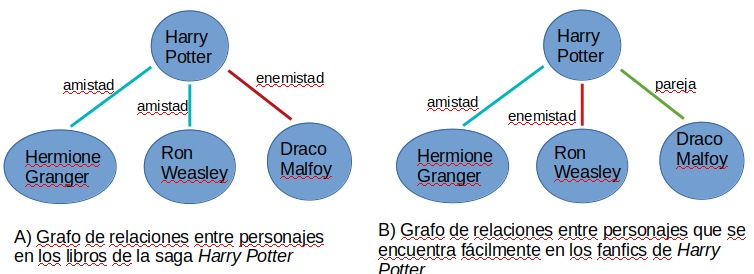
\includegraphics[scale=0.6]{rel_graph_hp2}
	\label{fig:graph_hp}
	\centering
\end{figure}


Como se ha dicho anteriormente, los fans se organizan en comunidades según la obra que es el objeto de su admiración, y tienen sitios como AO3, dedicados a alojar y compartir sus creaciones fan. Evidentemente, analizar las más de seis millones de obras existentes en AO3 es una tarea imposible con los recursos a mi alance, de modo que elegí utilizar únicamente los fanfics basados en \textit{Good Omens}, un libro de Terry Pratchett y Neil Gaiman, en parte por mi familiaridad con esa comunidad, pero también porque tenía una cantidad de fanfics extensa pero manejable.

AO3 no es el único sitio web popular para alojar fanfiction, pero a lo largo de esta década ha desplazado a sitios como \href{http://fanfiction.net}{Fanfiction.net} y \href{https://www.wattpad.com/}{Wattpad}, y la característica que condicionó mi decisión es su extensivo sistema de etiquetas, que como se verá más adelante fue fundamental para filtrar y gestionar los datos del proyecto.

En términos legales y de derechos de autor, la mayoría de legislaciones considera el fanfiction como un tipo de obra derivada \cite{woosh_1998} y por tanto entra dentro del \textit{fair use}.


\section{EXTRACCIÓN DE INFORMACIÓN EN OTROS TRABAJOS}

La identificación de entidades y relaciones son problemas que se abordan en el análisis de lenguaje natural, y en las últimas décadas han surgido diversas técnicas de \textit{machine learning} que han dado muy buenos resultados, sobretodo teniendo en cuenta la amplitud del tema. Es una solución atractiva por su capacidad de resumir y sacar conclusiones a partir de grandes volúmenes de textos ya existentes sin tener que dedicar grandes cantidades de tiempo y esfuerzos a leerlos manualmente, especialmente en campos como la medicina, en el que cada año se publica tal cantidad de estudios que es difícil mantenerse al día con los avances de ciertos campos.

La extracción de relaciones tradicionalmente se ha realizado tratando de identificar relaciones binarias, bien frase a frase o teniendo en cuenta dos o tres frases consecutivas\cite{zelenko_2003} \cite{craven_99}. Las limitaciones de este sistema no son sólo que no todos los tipos de relaciones son binarias, si no que cuanto más largo es un texto, menos probable es que ambas entidades aparezcan nombradas en una única frase, con lo que se pierde mucha información si se ignoran. Pasar a un sistema que tenga en cuenta varias frases interdependientes viene con sus propios problemas, pues las características sintácticas de una relación son muy dispersas en el texto y tratar de extraerlas automáticamente requiere de mucha memoria y muchos datos; más cuántas más frases tengas en cuenta. Sin embargo, recientemente se han creado algoritmos que identifican una relación n-aria a partir de todas las menciones en las que aparece, como el de Peng et al\cite{peng_17}, que utiliza grafos LSTM para modelar el contexto e información de cada frase y las conexiones entre ellas, logrando así beneficiarse de la interdependencia de distintas frases sin tanto coste de recursos.

Este proyecto sin embargo busca identificar relaciones de naturaleza social entre distintos personajes de ficción, con ĺo que serán relaciones binarias entre entidades exclusivamente del tipo 'Persona'. 
%El procesado de textos en lenguaje natural es una de las preocupaciones de la inteligencia artificial, y del aprendizaje automático en particular. 

%Otras aplicaciones similares a la mía: resumir texto?
% ontología star trek: \href{https://pr-owl.org/basics/ontostartrek.php}{ontología star trek}




\section{RECOGIDA Y LIMPIEZA DE DATOS}

\subsection{Creando un scraper para Archive of our Own}
\label{sec:recogidadatos}

En el momento en el que decidí utilizar los fanfics de \textit{Good Omens} para el proyecto, dicho libro tenía unos 22000 fanfics en \href{archiveofourown.org}{Archive Of Our Own} (AO3 para abreviar). Sin embargo, de todos esos relatos sólo me interesaban los que están en inglés y los que realmente contuvieran texto (puesto que, aunque AO3 se centra en relatos, permite alojar todo tipo de archivos multimedia).

Por suerte, AO3 fue creado con la intención específica de funcionar como archivo, por lo que tiene una herramienta de búsqueda y filtrado muy completa y sencilla de usar. Esta herramienta permite filtrar por características como título, autor, idioma y cantidad de palabras, pero su mayor utilidad viene de su sistema de etiquetado. AO3 permite a los autores añadir tantas etiquetas como quieran para que los posibles lectores puedan saber más de su obra a simple vista: temática, personajes principales, parejas en las que se centra, qué medio utiliza, si hay ilustraciones, si trata sobre un evento de la historia original particular... Las etiquetas añaden una gran cantidad de información sobre las historias a las que acompañan, y aunque no es obligatorio poner ninguna, en general los autores se preocupan de etiquetar correctamente sus obras.

\begin{SCfigure}
	\caption{Herramienta de filtrado de AO3. Permite excluir (o incluir) obras que contengan etiquetas específicas, así cómo aquellas no escritas en un idioma particular}
	\label{fig:ao3_search}
	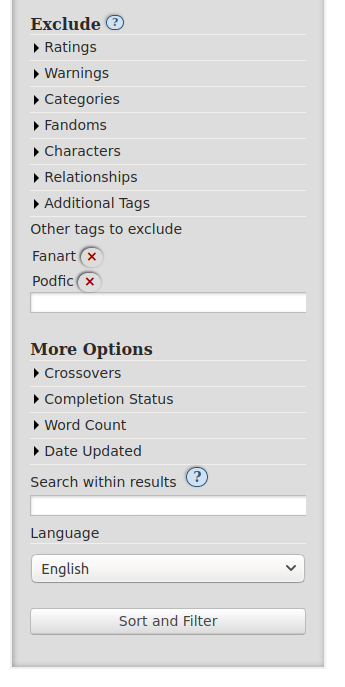
\includegraphics[scale=0.5]{ao3_searchbox}
	\centering
\end{SCfigure}

AO3 tiene etiquetas específicas para indicar que una obra no es principalmente texto: \textit{'Fanart'}, para ilustraciones, y \textit{'Podfic'} para archivos de audio, así que aproveché la herramienta de búsqueda para llevar a cabo un primer filtrado que eliminara todas las obras que las contuvieran, además de todas las que no estuviesen en inglés. El resultado fue un subconjunto de 20190 fanfics, todos en inglés y cuyos autores no habían incluido ninguna etiqueta que indicara que no fuera puro texto. La herramienta además genera un link permanente que siempre lleva a este subconjunto particular, por lo que no es necesario utilizar esta herramienta nada más que una vez.

\begin{figure}
	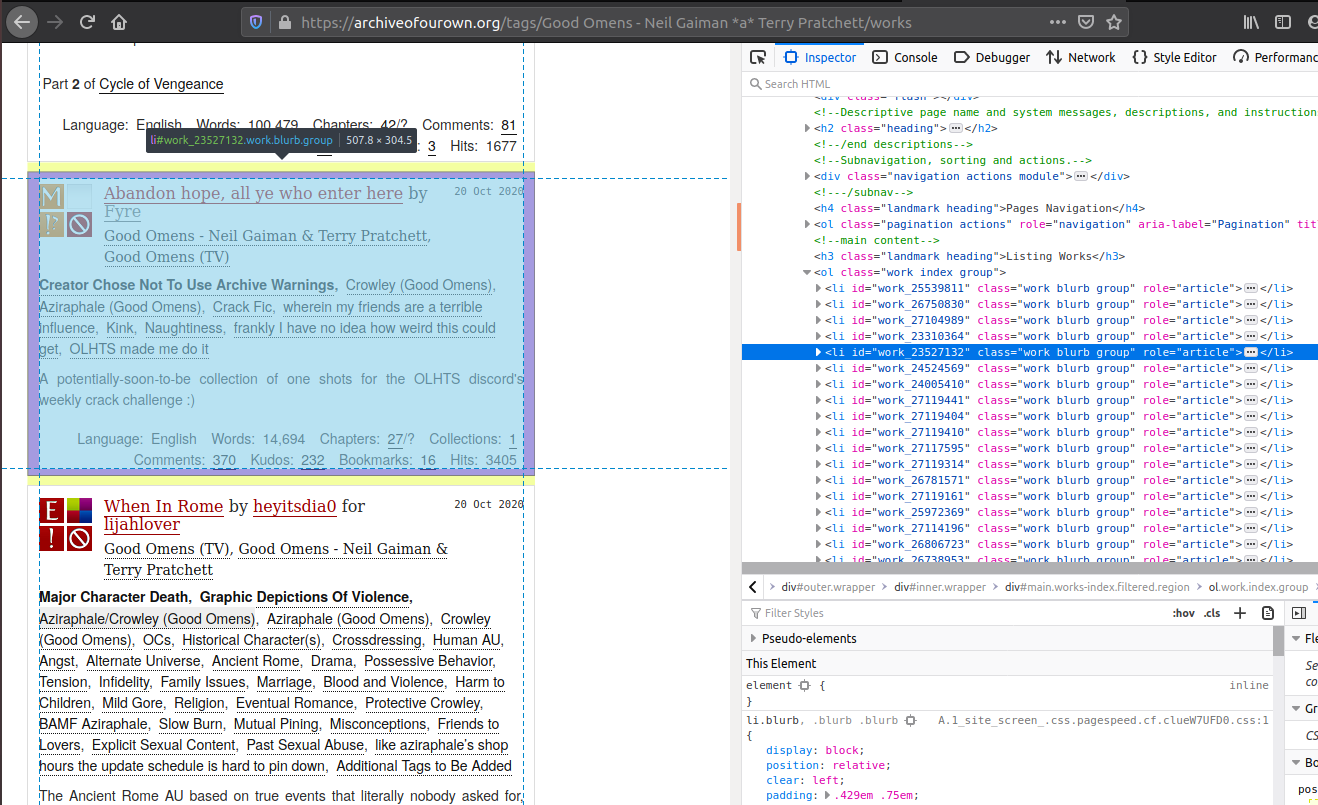
\includegraphics[angle=90,scale=0.5]{ao3_inspect}
	\caption{Exploración de la estructura de la página AO3 usando la herramienta 'Inspeccionar elemento' de \textit{Firefox}. Se puede ver que el sitio utiliza una clase HTML llamada \textit{'work blurb group'} para mostrar cada obra.}
	\label{fig:ao3_inspect}
	\centering
\end{figure} 

Una vez localizado el conjunto de textos y el link a los mismos, viene la parte de crear el \textit{scraper} en sí. Utilizando la herramienta de inspeccionar elemento de \textit{Firefox} para explorar la estructura del sitio, y enseguida se hizo obvio que los fanfics estaban organizados en páginas con un máximo de 20 fanfics cada una. En el HTML de la página, cada fanfic se presenta dentro de una clase llamada \textit{'work blurb group'}. No se puede extraer un link de descarga directamente de ésta clase, pero sí el identificador del fanfic.

En AO3, cada fanfic tiene un número que lo identifica de forma única. Es posible acceder a la página de cualquier fanfic simplemente añadiendo ese número al final de \newline 'https://www.archiveofourown.org/works/' en la barra de direcciones, y en esa página sí que se pueden encontrar links de descarga.

\begin{figure}[h]
	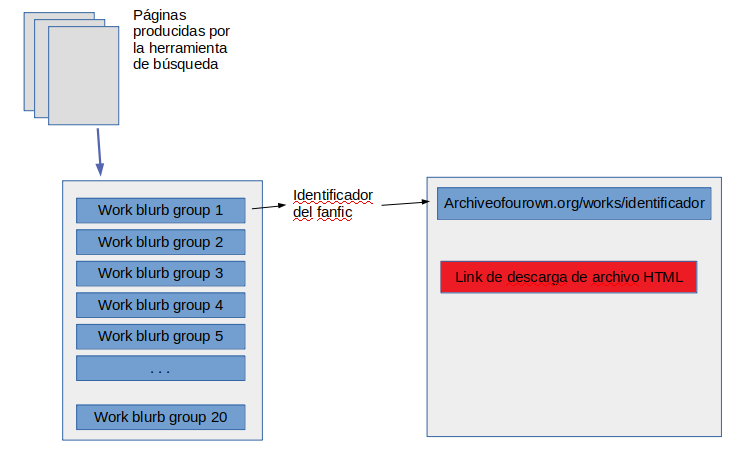
\includegraphics[scale=0.6]{ao3_structure}
	\caption{Concepto para el \textit{scraper}. El objetivo es obtener los links de descarga navegando las páginas de búsqueda.}
	\label{fig:ao3_structure}
	\centering
\end{figure}

Por tanto la idea básica para el \textit{scraper} es utilizar las librerías \textit{requests} y \textit{BeautifulSoup} de python para explorar los veinte \textit{'work blurb group'} de cada página, localizar el identificador de cada uno, utilizarlo para acceder a la página del fanfic y extraer el link de descarga. Y así con cada página del listado, hasta llegar a la última. La figura \ref{fig:ao3_structure} ilustra el proceso con un esquema.

El proceso de descarga de archivos, en principio, tendría estos pasos:

\begin{enumerate}
	\item Enviar una petición HTTP GET al link permanente del conjunto de datos, generado por la herramienta de búsqueda de AO3.
	\item Iterar entre los 20 \textit{'work blurb group'} y extraer el identificador de cada uno.
	\item Usar el identificador para acceder a la página de cada fanfic, extraer el link de descarga de la página, y descargar el fanfic como archivo HTML. Hacer esto con los 20 identificadores.
	\item Pasar a la siguiente página y repetir, hasta llegar a la última.
\end{enumerate}

Utilizando la librería \textit{requests} de python, el primer paso es trivial, y se puede observar en la figura \ref{code:scraper1}.

\begin{figure}
	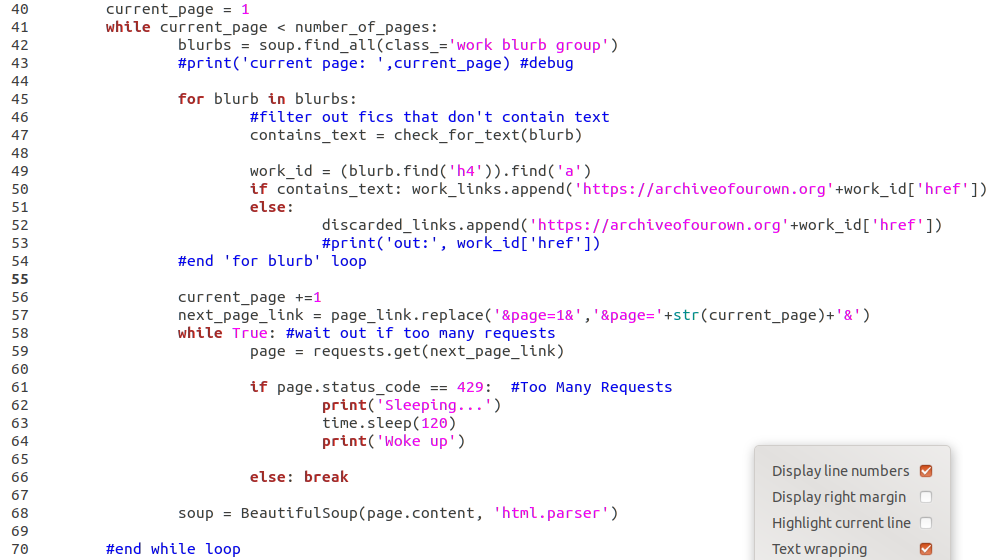
\includegraphics[scale=0.5]{scraper_code2}
	\caption{Código perteneciente al \textit{scraper} 'ao3\_link\_scraper'. Utiliza un bucle \textit{while} para iterar entre las páginas de la búsqueda, y en cada página, usa la librería \textit{BeautifulSoup} para extraer los objetos 'work blurb group' en una lista llamada 'blurbs' (línea 42). De cada 'blurb' extrae el identificador del fanfic y comprueba si tiene texto (líneas 46-49), y si lo contiene forma el enlace a la página del fanfic y lo añade a una lista llamada 'work\_links' (línea 50). Si no contiene texto, se añade a otra lista llamada 'discarded\_links' (línea 52).}
	\label{code:scraper2}
\end{figure}

Encontrar los identificadores tampoco es complicado. Se puede apreciar en \ref{fig:ao3_structure} que el identificador del fanfic también es el ID del objeto \textit{'work blurb group'} al que pertenece, y expandiendo la clase se puede ver que el identificador completo se puede encontrar dentro del objeto, como un objeto de tipo \textit{h4}. Por tanto, usando \textit{BeautifulSoup} para manejar los datos resultantes de la petición HTTP GET como objeto HTML, se pueden obtener todos los objetos \textit{'work blurb group'} usando la función \textit{find(class\_=<nombre clase>)}, cuyo resultado es una lista con los 20 objetos, sobre los cuales se itera para encontrar los identificadores usando de nuevo la función \textit{find()}. En la figura \ref{code:scraper2} se puede observar un fragmento del código que realiza este trabajo; el código completo se puede consultar en \refToLinkScraperCode.

Las complicaciones empiezan una vez se tienen los identificadores. Para formar la dirección completa, hay que añadir el identificador al final de \textit{'https://www.archiveofourown.org'}, mandar otra petición HTTP GET a dicha dirección, buscar ahí el link de descarga, solicitarla, esperar a que la descarga termine, y repetir todo esto otras 19 veces hasta tener descargados todos los fanfics de la página. Esto significa que por cada iteración del bucle que explora cada página es necesario introducir otro bucle que haga las descargas.

\begin{figure}
	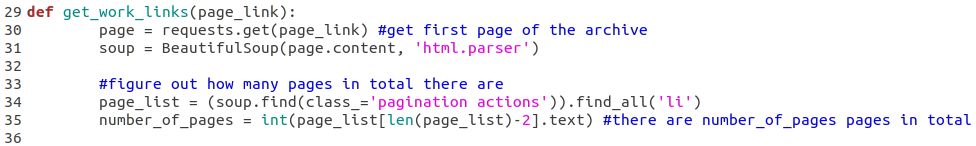
\includegraphics[scale=0.5]{scraper_code}
	\caption{Código perteneciente al \textit{scraper} 'ao3\_link\_scraper'. Utiliza la librería \textit{requests} para enviar una petición HTTP GET al link permanente del conjunto de datos (línea 30), y \textit{BeautifulSoup} para navegar el resultado como un objeto HTML del que poder extraer datos útiles, como la cantidad total de páginas (líneas 33-35).}
	\label{code:scraper1}
	\centering
\end{figure}

\begin{SCfigure}
	\caption{Navegación de páginas de búsqueda de AO3. Todos los botones vienen con su número de página, y se puede ver cuál es la última}
	\label{fig:ao3_structure2}
	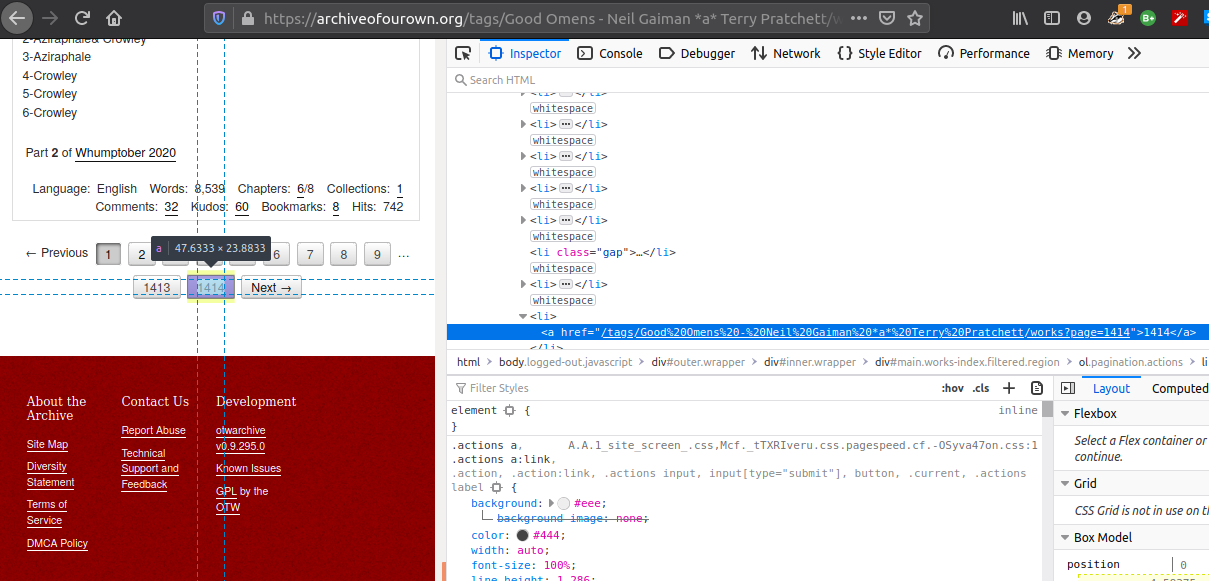
\includegraphics[angle=90, scale=0.5]{ao3_structure2}
	%\centering
\end{SCfigure}

La última parte, la de pasar a la página siguiente, es más complicada de explicar que de ejecutar. Todas las páginas de resultados de búsqueda de AO3 contienen botones para avanzar, retroceder y saltar a páginas concretas. Es posible saber cuántas páginas en total tiene la búsqueda simplemente observando el texto del botón de la última, tal y como se ve en la figura \ref{fig:ao3_structure2}. No se aprecia, pero la clase HTML a la que pertenece dicho botón se llama \textit{'pagination actions'}, y es posible extraerla gracias a la función \textit{find(class\_=<nombre\_clase>)} de \textit{BeautifulSoup}. Y ya con ese objeto, se puede volver a utilizar la función \textit{find()} para buscar todos los objetos hijos de la clase \textit{'pagination actions'} que sean de tipo \textit{li}. El último será el que contenga la cantidad total de páginas, y solicitar la siguiente consiste simplemente en sustituir la referencia en el link a la página 1 por una referencia a la última página. En la figura \ref{code:scraper1} se ve parte del código que realiza este proceso; el código completo se puede consultar en el anexo \refToLinkScraperCode.

Es evidente que la parte de solicitar las descargas en un bucle anidado ralentiza el programa, enturbia el código y además, hace que sea complicado parar o interrumpir el programa si hay algún error de red, pues para reanudar la ejecución por donde se quedó sería necesario almacenar en alguna parte el número de página por el que iba y el número del fanfic dentro de esa página, y programar los bucles para que salten directamente a la iteración deseada.

Ninguna de estas cosas me convenía, ya que descargar más de 20000 archivos ya iba a ser lento de por sí y hacerlo de una sentada sería prácticamente imposible, de modo que decidí dividir el programa en dos: uno que llamé 'link \textit{scraper}' y otro '\textit{file scraper}'.

\begin{figure}[h]
	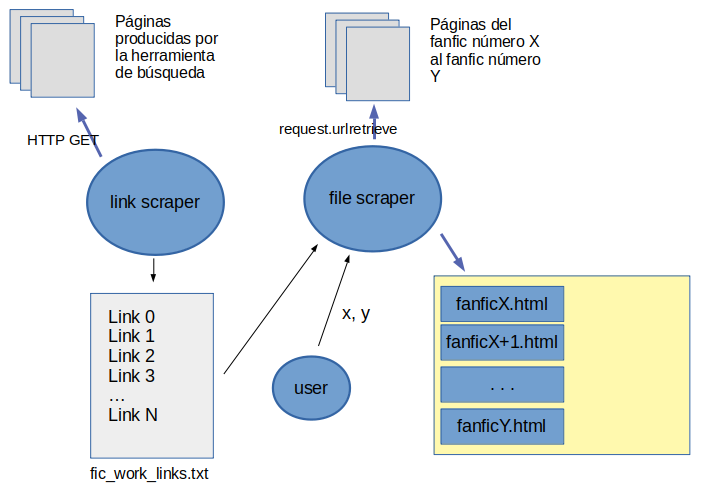
\includegraphics[scale=0.6]{scrapers_structure}
	\caption{Proceso de descarga de fanfics de AO3 utilizando los programas 'ao3\_link\_scraper.py' y 'ao3\_file\_scraper.py'.}
	\label{fig:scrapers_structure}
	\centering
\end{figure}

El link \textit{scraper} se ejecutaría una vez y exploraría todas las páginas de búsqueda, extrayendo los links a los fanfics de cada una, y los almacenaría en un archivo de texto. Por tanto, al terminar su ejecución este \textit{scraper} ha generado un archivo llamado '\textit{fic\_work\_links.txt}' que almacena los enlaces a cada fanfic. El \textit{file scraper} utiliza esta lista para saber dónde buscar las descargas, y el usuario le indica en la línea de comando los índices que acotan el tramo de la lista a descargar, tal y como se ilustra en el esquema de la figura \ref{fig:scrapers_structure}. De este modo, es posible indicarle al programa que descargue desde el link 0 al link 1000 de la lista, permitiendo descargar los 20000 archivos en porciones manejables. Además, el programa anuncia en pantalla qué link está siendo descargado en cada momento, por lo que si sucede un error de red mientras descargaba el link número 866, es posible reanudar el programa fácilmente e indicarle que continúe desde el 866 al 1000 \refToScraperExecution.

Esta división del trabajo en dos programas además me daba la oportunidad de introducir con sencillez un segundo filtrado durante el proceso de exploración que realiza el link \textit{scraper}. Si el primer filtrado se encargaba de cribar los fanfics que habían sido etiquetados por sus autores como imágenes o audio, este segundo filtrado pretende detectar los fanfics que tampoco contienen texto, pero no han sido etiquetados como tal por sus autores. Para ello usé el criterio de la relación palabras/capítulo de cada fanfic: si una obra tiene menos de 40 palabras por capítulo, se considera como fanfic "sin texto", y se elimina. Escogí 40 palabras como umbral tras investigar un poco con la herramienta de búsqueda de AO3, que como se puede ver en la figura \ref{fig:ao3_search}, tiene una opción para filtrar por cantidad total de palabras. Tras probar varios umbrales, 40 parecía ser el que descartaba todas las obras sin texto sin sacrificar muchos microrrelatos en el proceso.

Introducir este filtrado en el \textit{scraper} fue sencillo, puesto que el número de palabras y capítulos de la obra es información que se puede extraer de la clase \textit{work blurb group} de cada fic. Todo esto se realiza desde la función \textit{check\_for\_text}, y en la figura \ref{code:scraper2} se puede ver cómo el bucle llama a dicha función; el código completo se puede consultar en \refToLinkScraperCode. Por tanto, el link \textit{scraper} realiza estos pasos:
\begin{enumerate}
	\item Enviar una petición HTTP GET mediante la librería \textit{requests} al link permanente del conjunto de datos, generado por la herramienta de búsqueda de AO3.
	\item Iterar entre los 20 \textit{'work blurb group'}, comprobar si contienen texto, y descartar los identificadores de los que no.
	\item Utilizar cada identificador para generar el link de la página de cada fanfic y almacenarlos en un archivo de texto.
	\item Pasar a la siguiente página y repetir, hasta llegar a la última.
\end{enumerate}

\missingfigure{fig: pantallazo ejecución file scraper}

Por su parte, el \textit{file scraper} realiza estos pasos:
\begin{enumerate}
	\item Abrir el archivo \textit{fic\_work\_links.txt} y extraer la lista de links.
	\item Mediante la librería \textit{requests}, realizar una petición HTTP GET al primer link, saltando al siguiente si devuelve un código 404.
	\item Extraer el link de descarga HTML de cada página.
	\item Solicitar la descarga mediante \textit{request.urlretrieve}. Guardar el archivo resultante en la carpeta adecuada en el sistema.
	\item Repetir con todos los links de la lista.
\end{enumerate}

El manejo del código de error 404 (Page Not Found) es bastante importante en este \textit{scraper}, puesto que entre el momento en el que se almacenó el link del fanfic mediante el primer \textit{scraper} y el momento en el que el segundo \textit{scraper} lo utiliza para la descarga pueden haber pasado varios días. En ese tiempo, el autor del fanfic puede haber decidido borrar el fanfic de AO3, o haberlo hecho privado, y de ahí que el \textit{scraper} reciba un 404. Un simple \textit{try-catch} detecta el código 404 y simplemente pasa al siguiente link, como se puede consultar en el anexo \refToFileScraperCode.

El otro error que ambos \textit{scrapers} necesitaban manejar es, naturalmente, el error 429 (Too Many Requests). En las líneas 58-66 de la figura \ref{code:scraper2} se puede ver cómo se utiliza un \textit{try-catch} que envuelve la petición HTTP GET para detectar el status 429 y, en vez de pasar al siguiente link, se lanza una espera de dos minutos tras la cual vuelve a solicitar la página. Antes de incorporar este código a los \textit{scrapers} creé un pequeño programa de prueba, para ver cuánto tardaba AO3 en enviar un 429 y cuánto tiempo de espera requería antes de volver a aceptar solicitudes; dicho programa se puede consultar en \refToTrialCode.
 
%Decidí dividir este proceso en dos programas (el de navegación y filtrado, y el que únicamente descarga) en vez de hacerlo todo en uno porque descargar los más de 20000 archivos de una vez lógicamente tardaría varias horas, y pensé que sería más pragmático si ejecuto una vez el \textit{scraper} crea una lista de enlaces, y luego ya ejecuto todas las veces que sean necesarias el \textit{scraper} que descarga, descargando cada vez un tramo distinto de la lista. De esta forma, pude descargar todos los fanfics en grupos de 2000 (alrededor de una hora y media), pudiendo tener el ordenador libre el resto del tiempo.

El resultado de la ejecución de estos \textit{scrapers} es una carpeta con 818,8 MB de archivos HTML.

\subsection{Limpieza de datos y creación de datasets}
\label{sec:limpiezadatos}

Al terminar el proceso de descarga, acabé con un conjunto de archivos HTML y un archivo TXT con una lista de los \textit{path} de todos ellos.

La principal tarea de limpieza de datos es, por tanto, convertir los archivos HTML a texto. Para ello utilicé la librería \textit{HTML2Text}, que como cuyo nombre dice sirve para eso mismo. Sin embargo, los fanfics en HTML no contienen sólo el texto del fic en sí, sino que también contienen todos los metadatos del mismo: etiquetas, \textit{rating}, resumen, comentarios del autor, entre otros, con lo que tras limpiar el archivo HTML con \textit{HTML2Text} el resultado no era el texto puro del fanfic. Tuve que crear varias funciones y ayudarme de \textit{Beautiful Soup} para limpiar todos estos metadatos y dejar únicamente el texto en sí, sin llevarme por delante parte del texto ni dejarme notas del autor entre capítulos.

Al principio puse estas funciones dentro de cada programa que necesitaba manejar los textos, pero obviamente enseguida se volvió muy aparatoso, por lo que consolidé todas las funciones de limpieza en un único archivo, \textit{fanfic\_util.py}, junto con tres clases para encapsular el uso de estas funciones:

\begin{itemize}
	\item FanficGetter, que se encarga de proveer el texto limpio de un fanfic (o lista de fanfics) a demanda. Al principio devolvía los textos como una lista de \textit{string}, pero luego resultó más útil que devolviera una lista de objetos \textit{Fanfic} que pudiera devolver los capítulos por separado o juntos en un mismo \textit{string}, además del identificador del fanfic.
	\item FanficHTMLHandler se encarga de extraer información de los metadatos del archivo HTML de un fanfic, como por ejemplo los personajes principales, las relaciones, las etiquetas, el número de capítulos y su clasificación.
	\item Fanfic, una clase que se utiliza a lo largo del proyecto para encapsular toda la información relevante sobre un fanfic, como sus capítulos, sus personajes, etiquetas, el dataset al que pertenece e incluso los objetos \textit{Document} generados por CoreNLP.
\end{itemize}

La creación de la clase \textit{Fanfic} surgió a mediados del proyecto, cuando el límite de 100000 caracteres de \textit{CoreNLP}\ref{nota:limiteCarac} hizo necesario poder acceder al texto de cada fanfic dividido en capítulos. \textit{Fanfic} por tanto tiene un atributo \textit{chapters}, que es la lista de \textit{string} con los capítulos, y un método \textit{get\_string\_chapters()} que devuelve todos los capítulos en un único \textit{string}. Según seguía avanzando la clase también demostró ser útil para almacenar en un único elemento toda su información relevante, por lo que termina siendo la unidad básica de trabajo del proyecto.

\begin{figure}
	\centering
	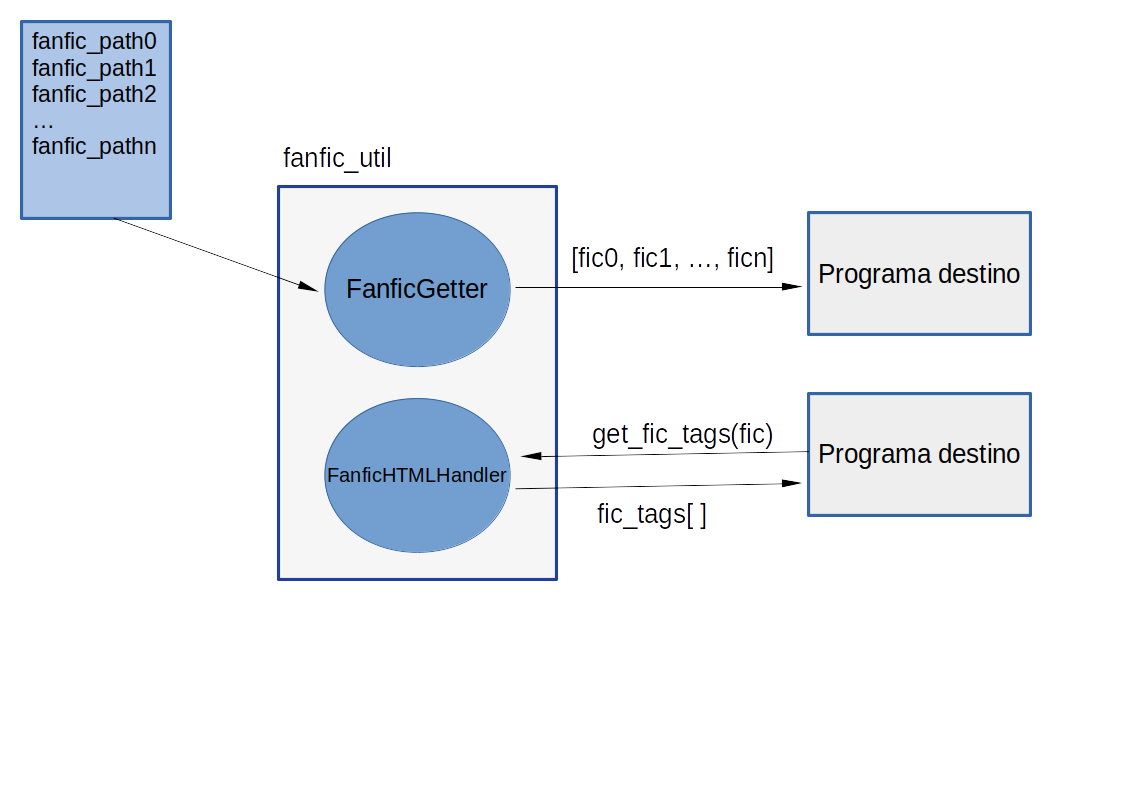
\includegraphics[scale=0.5]{fanfic_util_functions}
	\caption{Esquema ilustrando la función de las clases \textit{fanfic\_util}}
	\label{fig:fanfic_util}
\end{figure}

Sin embargo, el acceso a los datos sigue basándose en una lista de \textit{paths} guardada en un archivo TXT. Es un sistema muy rudimentario (ilustrado en la figura \ref{fig:fanfic_util}), pero no vi necesidad de trasladarlo a una base de datos propiamente dicha, puesto que nada en la creación de una base de datos me ahorraba nada del trabajo de crear \textit{fanfic\_util}, y desde el punto de vista del resto de programas es igual acceder al texto de un fanfic a través de FanficGetter que de una función que recupere el texto de una base de datos. Únicamente intercambiaría el tiempo de limpiar los textos por el de conectar con la base de datos y extraer su información.

El identificador de entidades puede utilizar la lista original con todos los fanfics como fuente para etiquetarlos, pero para la parte de identificación de relaciones del proyecto se necesita filtrar los fanfics originales en tres subconjuntos: uno centrado en el romance, otro en la amistad, y el último en la enemistad. Por lo tanto, utilicé las funciones de \textit{fanfic\_util} para crear un programa, \textit{generate\_fic\_lists.py}, para crear las listas de \textit{paths} correspondientes a cada grupo.

El criterio utilizado para crear estos tres grupos está basado en la longitud de los textos y sus etiquetas. En el caso de las etiquetas es sencillo: los autores casi siempre etiquetan las relaciones románticas en sus relatos, y a menudo también las amistades, para hacer que sus historias sean más fáciles de encontrar por aquellos que quieran leerlas. En AO3, las etiquetas románticas tienen el formato 'Personaje A/Personaje B', mientras que las etiquetas de amistad son 'Personaje A \& Personaje B' o 'Personaje A and  Personaje B', con lo que extraer estas etiquetas del archivo HTML es sencillo utilizando expresiones regulares \refToFilterCode. Además de tener una etiqueta que valide la expresión regular, sólo tuve en cuenta aquellos relatos que sólo tenían un capítulo. De esa forma, esperaba poder eliminar historias largas y elaboradas que contienen romance, pero que principalmente son una historia costumbrista o de aventuras. Limitando la longitud de la historia a un capítulo, todo el romance o la amistad queda condensada en dicho capítulo. Además, como en los relatos que contienen abusos sexuales es común etiquetar al perpetrador y a la víctima con el formato de 'Personaje A/Personaje B', realicé un segundo pase a la lista de romance, eliminando todos aquellos relatos que tuviesen la etiqueta 'Rape/Non-con'.

Crear un conjunto con relaciones de enemistad u odio es una tarea más complicada, ya que los usuarios de AO3 no tienen un formato oficial para las mismas y no se suelen etiquetar. Al final utilicé una lista de las etiquetas que los autores comúnmente utilizan como aviso de que su historia contiene violencia o abusos, como 'Rape/Non-con', 'Torture', 'Graphic Depictions of Violence' o 'Dead Dove: Do Not Eat'\refToFilterCode . Esperaba que, entre esas etiquetas y la limitación de longitud, pudiese aislar un conjunto de relatos que sirvieran de modelo para la relación de enemistad.

El resultado fueron 12520 relatos en el conjunto de romance, 784 en el de amistad y 155 en el de enemistad. Para equilibrar los \textit{datasets}, reduje el conjunto de romance a 220 y el de amistad a 180, dando un total de 555 relatos para modelar estas relaciones. A este \textit{dataset} lo llamo 'RFE dataset' (por \textit{Romance, Friendship, Enemy}) y se utiliza en la sección \ref{sec:relextract}.

\section {EXTRACCIÓN DE DATOS A PARTIR DE TEXTO}
\todo[size=\tiny]{Explicar los programas que hice para familiarizarme con NLTK}

En la identificación de entidades, se considera una entidad a los personajes, los lugares y las instituciones, entre otras cosas, que haya sido nombrada en el texto. Un algoritmo capaz de identificar entidades nombradas tiene que poder dividir un texto en tramos y asignarle una etiqueta de entidad ("Persona", "País", etc) a cada uno. Esta tarea además requiere que las palabras del texto hayan sido previamente etiquetadas con su rol morfológico.

Por estos motivos, la librería NLTK parecía la más idónea para la tarea. Es una librería de python que contiene herramientas básicas para el análisis de texto, y en particular me interesaba que venía con un \textit{part of speech tagger} (es decir, un identificador de rol morfológico) ya programado y entrenado. NLTK también viene con un identificador de entidades ya entrenado, pero quería programar uno que fuera más preciso y adaptado a mi conjunto de datos.



\subsection{Algoritmo de identificación de entidades}

\subsubsection{Extracción de entidades con NLTK}

Además del identificador de rol morfológico, NLTK también tiene una clase llamada \textit{ChunkParser} cuyo trabajo es dividir un texto en tramos. Todas las funciones de la librería que se encargan de dividir y/o etiquetar texto (como el identificador de rol morfológico) heredan de alguna versión de la clase \textit{ChunkParser}, de modo que la idea para el algoritmo era modificar la clase \textit{ChunkParserI} para convertirla en un identificador de secuencias basado en características. El código utilizado en este proyecto está basado en el tutorial de Ivanov en \textit{Natural Language Processing for Hackers} \cite{ivanov_2016}

Un identificador de secuencias basado en características trata de asignar un peso a un tramo concreto, y según el peso, le asigna una etiqueta u otra. Este peso se calcula como una función de las características del propio tramo, así como de los tramos que le preceden.
El programador puede elegir las características que considere más importantes, pero hay algunas que son bien conocidas como las más importantes para reconocer entidades, como:

\begin{itemize}
	\item El rol morfológico de la palabra actual, las anteriores y las siguientes.
	\item La forma de la palabra, las anteriores y las siguientes (si empiezan por mayúscula, si tienen signos de puntuación, si son siglas, etc)
	\item Los prefijos y/o sufijos de la palabra actual, las anteriores  y las siguientes.
	\item Si la palabra anterior ha sido identificada como una entidad o no.
	
\end{itemize}

El conjunto de características de cada tramo se llama vector de características, y se utiliza para calcular un "peso" que se corresponde con la probabilidad de que un tramo X con un vector de características V tenga una etiqueta Y. El algoritmo al final asigna a cada tramo la etiqueta cuyo peso sea el más alto.

El cómo se calcula exactamente ese peso depende del modelo matemático a utilizar. A la versión modificada de ChunkParserI para la identificación de entidades la llame NERChunker (NER por Named Entitiy Recognition), y tiene tres versiones:

\begin{itemize}
	\item NERChunkerv1 y NERChunkerv3 utilizan un modelo de regresión logística (también llamado modelo de entropía máxima), a través de la clase MaxentClassifier de NLTK. Para que NLTK pueda utilizar esta clase correctamente, es necesario tener instalado el módulo Megam para python, que no viene incluído en NLTK. La única diferencia entre la versión 1 y la 3 de este chunker es que la 3 maneja las estructuras de NLTK para oraciones y etiquetas de forma ligeramente más rápida.
	\item NERChunkerv2, que utiliza un modelo de naïve Bayes a través de la clase ClassifierBasedTagger de NLTK.
	
\end{itemize}

Las versiones \textit{v1} y \textit{v3} de \textit{NERChunker} obtuvieron los mejores resultados en la evaluación, y la \textit{v3} es algo más rápida, por lo que es la versión definitiva del identificador de entidades. Todas estas versiones, junto con sus funciones auxiliares, se encuentran encapsuladas en el archivo \textit{NERChunkers.py}, para ser utilizadas donde se las necesite.

Puesto que tanto los clasificadores de regresión logística como los de \textit{naïve} Bayes son algoritmos de aprendizaje supervisado, antes de poder utilizar (o evaluar) cualquiera de las versiones de \textit{NERChunker} era necesario entrenarlas con un conjunto de datos ya etiquetados. El problema aquí es que NLTK, a pesar de incluir un corpus muy extenso en la propia librería, sólo tiene dos conjuntos de datos para identificación de entidades: uno en español y el otro en holandés. Todos los textos a analizar en el proyecto están en inglés, obligándome a buscar un conjunto ajeno a NLTK y finalmente decidiéndome por \textit{Groningen Meaning Bank} (GMB). GMB es un \textit{dataset} para identificación de entidades específicamente en inglés, grande, con una gran variedad de etiquetas de entidad y, sobretodo, con un formato de etiquetado sencillo de entender,cosa importante puesto que al ser ajeno a NLTK, GMB utiliza etiquetas distintas que son necesario adaptar para que \textit{MaxentClassifier} pueda trabajar con ellas.

GMB utiliza la notación IOB para etiquetar entidades, y separa cada palabra de la siguiente por un carácter de nueva línea, y cada frase, por dos. De modo que la frase \textit{"Mr. Blair left for Turkey Friday from Brussels."} en GMB tendrá el aspecto de la figura \ref{fig:tags1}.

\begin{figure}[h]
	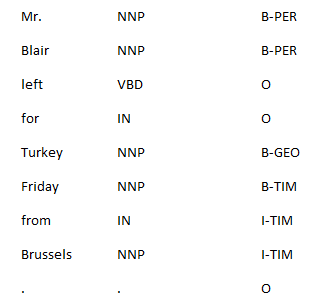
\includegraphics[scale=0.9]{GMB_tag}
	\caption{Frase etiquetada por GMB. De izquierda a derecha, las columnas representan la palabra a etiquetar, la etiqueta de rol morfológico, y la etiqueta IOB.}
	\label{fig:tags1}
	\centering
\end{figure}

Cuando el programa detecta una entidad de tipo persona, etiqueta como 'B-PER' la primera palabra de la secuencia, mientras que el resto de palabras dentro de la secuencia son etiquetadas como 'I-PER'. Similarmente, si la entidad es de tipo geográfico las etiquetas usadas serán 'B-GEO' y 'I-GEO', si es de tiempo serán 'B-TIM' y 'I-TIM', etc. Si una palabra no forma parte de ninguna secuencia de entidad, se etiqueta como 'O'.

NLTK, por su parte, no utiliza la notación IOB  ni caracteres de nueva línea, sino que utiliza una estructura de datos propia de tipo árbol que encapsula cada palabra y cada tramo con su etiqueta. La misma frase etiquetada por NTLK tiene el aspecto de la figura \ref{fig:tags2}.

\begin{figure}[h]
	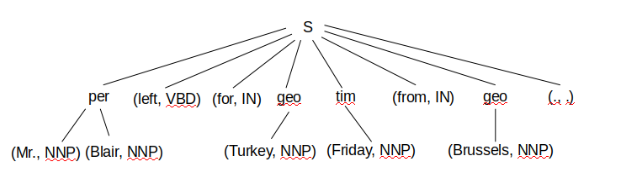
\includegraphics[scale=0.8]{NLTK_tag}
	\caption{Frase etiquetada por NLTK. Las etiquetas de entidad se encuentran en los nodos, encontrándose todas las palabras pertenecientes a una secuencia de entidad en la profundidad 2 del árbol. Las palabras que no pertenecen a ninguna secuencia de entidad se encuentran en la profundidad 1. Cada hoja del árbol contiene una tupla formada por la palabra y su etiqueta de rol morfológico.}
	\label{fig:tags2}
	\centering
\end{figure}

Como se ve, en vez de usar etiquetas IOB, NLTK organiza las palabras y su etiquetas en una estructura de árbol. La raíz, S, indica el inicio de la frase (Sentence), y las etiquetas de entidad son nodos.

En horizontal queda así:

(S, [(per, [(‘Mr.’, NNP), (‘Blair’, NNP)]), (‘left’, VBD), (‘for’, IN), (geo, [(‘Turkey’, NNP)]), (tim, [(‘Friday’, NNP)]), (‘from’, IN), (geo, [(‘Brussels’, NNP)]), (‘.’,.)])

Fue más o menos a estas alturas del proyecto cuando decidí separar el proceso de entrenar el identificador de entidades y el de utilizarlo para etiquetar texto nuevo en dos programas distintos (NERTrainer y NERTagger, respectivamente). Acceder a los textos de GMB y transformar sus etiquetas a un formato que NLTK pueda entender y acceder a los textos de la base de datos de fanfics y preprocesarlos para su posterior etiquetado mediante el programa ya entrenado han resultado ser dos procesos muy distintos, y dividirlo parecía la mejor manera de tener un código limpio y claro.

Por lo tanto, el programa \textit{NER\_trainer.py} se encarga únicamente de entrenar el \textit{chunker} y guardarlo en un objeto binario con la ayuda de \textit{pickle}, mientras que el programa \textit{NER\_tagger.py} carga el objeto binario y lo encapsula en una clase NERTagger, de modo que cualquier otro programa pueda utilizarlo cuando lo necesite.

\begin{figure}
	\centering
	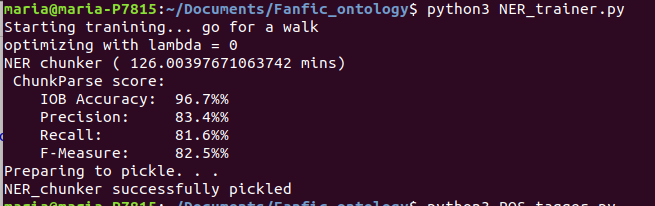
\includegraphics[scale=0.6]{ejecucion_nertrainer}
	\caption{Ejecución final de \textit{NER\_trainer.py}, mostrando su evaluación.}
	\label{fig:ner_evaluation}
\end{figure}

%%% DETALLES TÉCNICOS %%%
% POS\_tagger.py: para poder etiquetar las entidades nombradas es necesario etiquetar cada palabra con su rol morfológico, de modo que este programa se encarga de abrir los archivos html, pasarlos a texto y ponerle sus etiquetas morfológicas. Para ello utiliza los métodos de NLTK word\_tokenize y sent\_tokenize para dividir cada texto en frases y palabras, y pos\_tag para usar el clasificador por defecto de python para asignar etiquetar morfológicas en inglés. Almacena el resultado en un csv, de modo que en vez de tener preparar el archivo html y etiquetarlo cada vez que quiera identificar entidades, sólo tengo que etiquetar cada archivo una vez.
% NER\_trainer.py: entrena el algoritmo identificador de entidades usando el dataset de entrenamiento (descargado de aquí) y guarda el objeto en un archivo binario usando la librería pickle. Una vez entrenado, evalúa la precisión del algoritmo y la imprime por pantalla. Como el dataset no es parte del corpus nativo de NLTK, mucho de éste programa consiste en abrir el csv del dataset y empaquetar sus datos en listas y tuplas que sean compatibles con NLTK, y dividir el resultado en un dataset de entrenamiento y dos para hacer test (80\%, 10\% y 10\% del dataset original, respectivamente). Este programa utliza un objeto de la clase NERChunkerv1, que se encuentra en el archivo NER\_chunker.py, que se explica más abajo.
% NER\_tagger.py: utliza la libraría pickle para deserializar el archivo binario entrenado por NER\_trainer.py, y lo utiliza para etiquetar entidades nombradas en frases (usando etiquetas IOB). Utiliza el archivo csv creado por POS\_tagger para saltarse la parte de asignar etiquetas morfológicas, y guarda sus etiquetas en otro csv, de modo que gran parte de su código se dedica a lidiar con abrir, leer y actualizar archivos csv.


%En NERChunkerv1 he utilizado una interfaz de NLTK llamada ChunkParserI. Tiene el constructor y dos métodos:
%\begin{itemize}
%	\item el constructor recibe el dataset en forma de frases etiquetadas y entrena el algoritmo. El dataset que he utilizado venía con etiquetas IOB en forma de tuplas, pero NLTK usa las etiquetas IOB en otro formato, de modo que el constructor se dedica principalmente a manipular las tuplas y aplicarles el método tree2conlltags para que NLTK las entienda. Y después llama a NERTagger y le pasa el dataset ya preparado para entrenar un clasficador.
%	\item parse, que es el método que recibe una frase con etiquetas morfológicas y la etiqueta, con el clasificador ya entrenado. Devuelve la frase etiquetada con etiquetas IOB en forma de árbol, que es el formato de etiqueta que NLTK utiliza.
%	\item evaluate, que evalúa la precisión del algoritmo. Uso el de laIdentificación de eventos superclase, así que en mi código no está definido.
%\end{itemize}


%NERTagger mantiene un historial de etiquetas IOB (una lista) y depende de feature\_function, una función que recoge ciertas características (featureset) de una palabra y las devuelve en forma de diccionario. Las características que recoge son éstas:

\subsubsection{Extracción de entidades con CoreNLP}
La decisión de incluir CoreNLP en el proyecto está motivada por la posibilidad de no sólo aprovechar sus capacidades para identificar menciones a una entidad en un texto, y, sobretodo, su función de resolución de correferencia para identificar relaciones entre personajes en un texto. En la sección \ref{sec:correferencia} está explicado en mayor detalle por qué esto podría ser relevante para el proyecto y cómo utilizarlo en python, pero aquí baste con mencionar que la resolución de correferencia es un método por el cual se enlaza un pronombre con el nombre propio al que se refiere. Por ejemplo, en una frase como \textit{'I love you, Juliet'} se podría aplicar correferencia para enlazar el \textit{you} con \textit{Juliet}. En este ejemplo, \textit{you} es una mención pronominal, mientras que \textit{Juliet} es una mención propia.

Esto hace que CoreNLP sea una un complemento atractivo al NERtagger desarrollado en la sección anterior, ya que además del nombre del personaje también recoge información de sus pronombres, posibilitando identificar su género y llevar una cuenta más precisa de cuántas veces se menciona un personaje concreto en el texto (incluso aunque la mención sea sólo un pronombre como \textit{he}). En esta sección se explica cómo utilizar todas estas funciones, además de los metadatos a nuestra disposición, para identificar y extraer el nombre y el género de los personajes presentes en un texto. Además, puesto que la intención del programa es que el fanfic se pueda comparar con el texto original en el que se basa, por cada personaje se identificará si aparece en la obra original o es un añadido del autor fan.

La idea básica para la extracción de personajes es buscar tanto las menciones de entidad como las de correferencia (en particular, las menciones pronominales y propias).
Como se explica en su \href{https://github.com/stanfordnlp/stanza/blob/master/doc/CoreNLP.proto}{documentación}, CoreNLP tiene dos tipos de menciones:
\begin{itemize}
	\item \textit{NERMention}, para las menciones relacionadas con identificación de entidades. Hay varios tipos, pero este proyecto se utiliza sobretodo las menciones de tipo 'PERSON'. Cada mención tiene un entityMentionIndex que la identifica de forma única, y además también tiene un canonicalEntityMentionIndex que identifica a la entidad particular a la que hace referencia (de modo que si una entidad se llama John Smith, todas las menciones que contienen John irían idexadas a una única NERMention).
	\item \textit{Mention}, para las menciones de correferencia. En este proyecto se utilizan sobretodo las de tipo 'PROPER' y 'PRONOMINAL', ya que son las que identifican nombres y pronombres. Cada una tiene un mentionID que la identifica de forma única, además de un corefClusterID y un goldenCorefClusterID que indican los clusters a los que pertenecen.
\end{itemize}

Una vez procesado un texto, CoreNLP devuelve un objeto \textit{Document} que contiene todos los NERMention y Mention detectados en el texto. Es sencillo hallar los personajes simplemente creando una lista que contenga todas las NERMention con un mismo canonicalEntityIndex, pero todas estas menciones contienen el nombre o parte del nombre de un personaje, y mi intención era hallar también los pronombres utilizados para referirse a un personaje. Ahí es donde entra la función de resolución de correferencia, cuyo resultado se almacena en las Mention: una mención de tipo PROPER contiene el nombre de un personaje, mientras que las de tipo PRONOMINAL contienen algún pronombre. CoreNLP organiza todas estas menciones en clusters, de modo que una mención PROPER y una mención PRONOMINAL comparten el mismo cluster si se refieren a la misma entidad. Para decidir en qué cluster debe ir una mención, CoreNLP tiene en cuenta factores como el género identificado de la entidad, la distancia entre menciones y cuál fue la última entidad mencionada.

La estrategia más evidente es hacer una lista con todas las menciones PROPER y PRONOMINAL, identificar sus clusters y asociarlos a las entidades de las NERMentions, de modo que por cada texto se tenga una lista de personajes únicos con su identificador, su nombre y su género.

Sin embargo, antes incluso de empezar a entender cómo se relacionan las Mention y NERMention con el texto, hay que tratar el problema de la latencia de CoreNLP, y es que es un servidor que realmente no está preparado para procesar grandes cantidades de información. Mis primeros programas manejando CoreNLP podían tardar alrededor de un minuto por texto, lo cual no es un problema terrible para procesar uno o dos textos, pero puesto que la intención inicial de utilizar CoreNLP era analizar un dataset de casi 400 textos (sección \ref{sec:correferencia}) me vi obligada a buscar una forma eficiente de realizar las peticiones. Además, muchos de los textos exceden el límite de 100000 caracteres del servidor, lo cual hace que la petición expire y el servidor se cierre, terminando el programa. Aunque es posible aumentar dicho límite con los parámetros de configuración del servidor, la mejora en rapidez es insuficiente.

El límite de caracteres tiene fácil solución, puesto que basta con enviar cada fanfic como una lista de capítulos \label{nota:limiteCarac} (dividiendo aquellos que aún sigan excediendo el límite), y cada capítulo se envía en un petición separada. Obviamente eso significa que por cada texto se pueden recibir dos o más objetos \textit{Document}, lo que significa que un mismo personaje puede tener distintos identificadores según el \textit{Document} en el que se generó su mención, lo que complica ligeramente el proceso de consolidación de personajes, como se explica más adelante. Sin embargo, esta división del texto en distintas peticiones evita con éxito que expiren por ser demasiado grandes, pero la respuesta sigue siendo muy lenta para listas de más de 9 ó 10 textos, dependiendo de lo largos que sea cada uno.
Finalmente la solución fue rediseñar el programa de manera que en vez de abrir y cerrar el servidor por cada texto, se abre una vez y todas las peticiones se envían juntas. Aunque el tiempo que se tarda en abrir el servidor casi siempre es menor que el necesario para procesar el texto en sí, era obviamente la manera más simple de ahorrar tiempo de ejecución.

Para facilitar todo este proceso se crea la clase CoreWrapper \todo{cambiar a CoreClient si necesario}, que se encarga de todo lo relacionado con la comprobación del límite de caracteres y manejar el servidor. CoreWrapper simplemente recibe una lista de objetos Fanfic y devuelve esencialmente la misma lista, pero ahora cada Fanfic tiene un atributo \textit{annotations} que es una lista de los \textit{Document} asociados a él.
CoreWrapper también maneja los errores de servidor y de red que puedan ocurrir durante la ejecución de CoreNLP, avisando si uno se produce, y asegurando que los datos obtenidos hasta el momento sean almacenados. Ésta función resultó muy importante en el procesado del RFE dataset en la sección \ref{sec:correferencia}, puesto que CoreNLP es bastante propenso a errores de red y rara vez podía digerir más de 25 fanfics de golpe. 

Una vez solucionado el problema de la latencia, el siguiente reto es entender cómo CoreNLP indexa cada palabra u oración de un texto con sus correspondientes menciones, y cómo éstas se refieren unas a otras. Repasé la documentación de CoreNLP, además de dibujar esquemas y crear varios programas para encontrar el mejor método de agrupar Mention en clusters y NERMention en listas que contuvieran toda la información necesaria para identificar cada personaje. Tras toda esta experimentación, todas las menciones y su información quedaron resumidas en listas de diccionarios de python, de forma que cada diccionario representa una mención e incluye el texto de la mención (que generalmente es el nombre del personaje), el género del personaje, y otra información como el tipo de mención y sus identificadores (de entidad, de cluster, etc).

\missingfigure{fig: esquema de indexación de corenlp}

Puesto que las menciones de correferencia pertenecen a clusters de menciones, mientras que las menciones de entidad tienen un identificador, en un principio pensé en clasificar todas las menciones de correferencia según cluster, determinar qué personaje representa qué cluster y luego asociar cada uno de estos clusters con un los identificadores de entidad, teniendo en cuenta factores como el género y el  nombre de cada uno.
Sin embargo, los clusters de correferencia no se corresponden fácilmente con personajes, especialmente si dos personajes del mismo género aparecen mencionados juntos (cosa a la que éste conjunto de relatos es muy susceptible). Por tanto, para consolidar las menciones de correferencia en personajes tuve aprovechar otros patrones en la información proporcionada por CoreNLP:

\begin{enumerate}
	\item A veces las menciones de entidad y las de correferencia coinciden en una misma palabra. En particular, las menciones de tipo 'PROPER' (que corresponden con sustantivos y nombres propios) como mínimo a veces también serán una mención de entidad.
	\item Las menciones de correferencia tienen un atributo \textit{headString}, que es la palabra que CoreNLP identifica como la más importante en la mención, y que suele corresponderse con el nombre propio del personaje (si una mención es 'Mr. Smith', por ejemplo, CoreNLP identifica 'Smith' como el \textit{headString} de la mención).
	\item Cuantas más menciones tenga un personaje, más probable es que dicho personaje sea un personaje real en el texto, y no un error de identificación.
\end{enumerate}

%\missingfigure{fig: analisis corenlp}

\begin{figure}
	\centering
	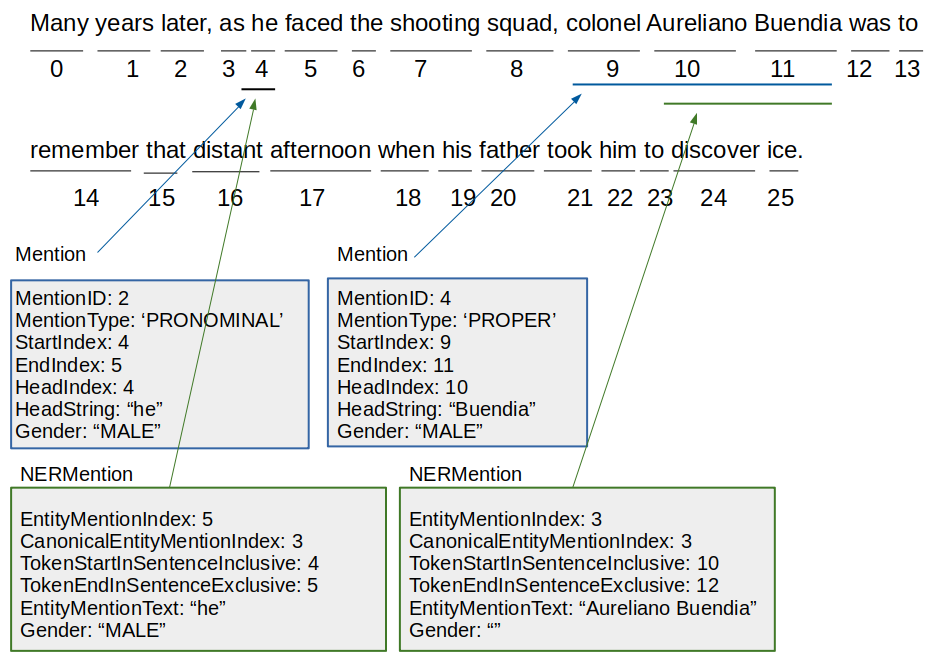
\includegraphics[scale=0.5]{solapamiento_esquema}
	\caption{Solapamiento entre menciones de correferencia (Mention) y de entidad (NERMention).}
	\label{fig:solapamiento_esquema}
\end{figure}

En base a estas observaciones se pueden determinar algunas reglas para decidir qué menciones se refieren a qué personaje:

\begin{enumerate}
	\item Todas las NERMention que tengan el mismo \textit{canonicalEntityMentionIndex} se consideran como el mismo personaje, y el atributo \textit{entityMentionText} se considera el nombre del mismo.
	\item Identificar las Mention que también son menciones de entidad. Dichas Mention se consideran como el mismo personaje que el de la NERMention.
	\item De las Mention que hayan podido ser identificadas como pertenecientes a un personaje, obtener su cluster de correferencia y considerar a todas las Mention de dicho cluster como pertenecientes a dicho personaje, pero sólo si 1) El atributo \textit{gender} de ambas menciones son el mismo, y 2) El atributo \textit{headString} de ambas Mention tienen una distancia de edición menor que 3 (para evitar descartar posibles errores tipográficos).
\end{enumerate}

El resultado de este proceso es una lista de diccionarios de python que representan personajes, conteniendo su nombre, su género, el número de veces que es mencionado, a qué clusters pertenece, etc.

Esta lista aún es bastante imperfecta. De entrada, los identificadores de entidad y de cluster asignados a cada mención dependen del \textit{Document}, y dada la estructura del programa, la mayoría de relatos van a tener asociados dos o más \textit{Document}, lo que significa que hay personajes con exactamente el mismo nombre y género que aparecen como dos personajes distintos, porque no comparten el mismo \textit{canonicalEntityMentionIndex} ni ningún cluster de correferencia. Además, esta forma de identificar personajes significa que si alguno tiene un apodo, o si a un personaje se le llama de forma consistente por su apellido en una zona del texto y por su nombre en otro, aparecerá como dos personajes distintos. Para mitigar estos errores, implementé un paso de canonicalización de personajes.

Vamos a aprovechar el hecho de que los relatos que estamos manejando pertenecen al género fanfic, es decir, son obras basadas en obras ya existentes. Eso quiere decir que hay una alta probabilidad de que la mayoría o incluso todos los personajes del fanfic no sean creación del autor, sino que ya aparecían en la obra original. A estos personajes se les llama 'personajes canon'.

En este proyecto, la canonicalización de personajes consiste en descubrir qué personajes del fanfic son canon o no. Para ello necesito la lista de personajes que sí que son canon, de modo que, con la ayuda de \href{https://goodomens.fandom.com/wiki/Category:Characters}{la página de personajes de la wiki de \textit{Good Omens}}, creo un archivo llamado \textit{canon\_characters.csv} que sirve como base de datos de los personajes de la obra original, asignándole a cada uno un identificador numérico. La base de datos además también contiene el género canónico de cada personaje, y una lista con sus apodos.

Durante la canonicalización también vamos a determinar el género de un personaje de forma definitiva, y para ello vamos a aprovechar nuevamente que estamos manejando fanfics y que, por lo general, los autores etiquetan sus fanfics. No todos ellos etiquetan el género de sus personajes, pero algunos sí, ya que hay personas a las que le gusta explorar la personalidad o sexualidad de los personajes mediante técnicas como cambiarles el género o darles una expresión ambigua. Algunos ejemplos de las etiquetas que se suelen usar para indicar el género de un personaje son 'He/Him Pronouns for Crowley', 'Androgynous Crowley' o 'Female!Crowley'.

Teniendo en cuenta todos estos factores, la canonicalización de un personaje consiste en estos pasos:
\begin{enumerate}
	\item Identificar si es canon o no:
	\begin{enumerate}
		\item Comprobar si el nombre del candidato a personaje tiene una distancia de edición menor que 2 con el nombre canon de algún personaje. Si lo hay, el candidato se considera ese personaje del canon.
		\item Si no coincide con el nombre del personaje canon, se pasa a hacer la misma comprobación con los apodos conocidos del mismo. Si coincide con alguno, el candidato se considera ese personaje del canon.
	\end{enumerate}
	
	\item Identificar el género del personaje:
	\begin{enumerate}
		\item  Obtener las etiquetas su fanfic y comprobar si hay alguna etiqueta que indique el género del personaje. Si la hay, el personaje se considera de ese género.
		\item Si no hay ninguna etiqueta, nos quedamos con el género que CoreNLP le haya asignado.
		\item Si CoreNLP no le ha asignado ningún género ('UNKNOWN', o simplemente el \textit{string} vacío ''), le asignamos el género del personaje canon. Por tanto, si el personaje no es canon, su género seguirá siendo desconocido.
	\end{enumerate}
\end{enumerate}

Este proceso resuelve los problemas relacionados con tener los mismos personajes procesados en distintos \textit{Document}, y asegura que una mención será identificada con el personaje canon tanto si menciona el nombre, el apellido o sólo un apodo. Además, este proceso sigue siendo capaz de identificar correctamente a un personaje con su correspondiente en el canon aunque el género no concuerde, e incluso si el personaje cambia de género durante la historia.

Todos este proceso de extracción de personajes se lleva a cabo mediante una clase CoreNLPDataProcessor, que se encuentra encapsulada junto a CoreWrapper en un programa llamado \textit{corenlp\_util.py}. CoreNLPDataProcessor, además de extraer personajes, también tiene función de análisis de sentimiento, como se explicará en la sección \todo{ref a programa principal}.

En la figura \ref{fig:extraccionPersonajes} hay un esquema que explica de forma visual todo este proceso de extracción de personajes.

\missingfigure{fig:esquema extracción personajes}


\todo{explicar posibles problemas y carencias de este proceso (apodo que es un sustantivo común como "ángel", posibles confunsiones entre un Mr Smith con Ms Smith)}

\subsection{Algoritmo de identificación de relaciones}

Las relaciones que definen un fanfic son las amistades, los enemigos y, principalmente, los amantes. Extraer relaciones a partir de texto natural es una tarea compleja de por sí, y tratar de detectar este tipo concreto de relaciones en literatura de género puede presentar un reto mayor, puesto que las relaciones sentimentales tienden a representarse de forma implícita, de modo que el lector aprende quiénes son amigos y quiénes enemigos a través de las acciones de los personajes. Además, la ambigüedad, la heterogeneidad y la experimentación son partes naturales de cualquier proceso creativo, por lo que un conjunto de obras no representará una misma relación de forma uniforme, incluso si es entre los mismos personajes.

Encontrar una estrategia para abordar este problema requiere exploración y creatividad, y ya que había empezado el proyecto con NLTK, me pareció natural comenzar la búsqueda por ahí.

El extractor de relaciones de NLTK funciona mediante reglas: después de extraer las entidades nombradas del texto, se puede utilizar el módulo \textit{relextract} para dividir el texto en listas de fragmentos del texto que contienen dichas entidades, y aplicar reglas basadas en expresiones regulares que definan la relación entre las entidades. La regla puede incluir etiquetas de rol morfológico en la expresión regular, y \textit{relextract} permite filtrar por etiqueta IOB, lo que le da algo más de flexibilidad.

Por ejemplo, para extraer una relación de lugar entre una organización y una localización, se puede crear una expresión regular que busque la palabra clave 'in' en el texto, e indicarle a \textit{relextract} que sólo te interesan los fragmentos de texto que tengan una entidad de tipo 'ORG' seguida de una entidad de tipo 'LOC':
\begin{lstlisting}[style=consola, caption=Ejemplo de código que utiliza el módulo \textit{regexp} de NLTK para extraer relaciones de lugar y mostrarlas por pantalla. Adaptado del capítulo 7 de Natural Language Processing with Python\cite{bird_2012}]
IN = re.compile(r'.*\bin\b(?!\b.+ing\b)')

for doc in parsed_docs:
	for rel in nltk.sem.extract_rels('ORG','LOC', doc, pattern=IN):
		print(nltk.sem.show_raw_rtuple(rel))

\end{lstlisting}

Existen proyectos que utilizan este módulo de NLTK para extraer relaciones como \textit{DateOfBirth} y \textit{HasParent} \cite{jose_2017}, pero es evidente que es un método poco adecuado para el tipo de proyecto que estaba intentando hacer.

Estos programas basados en reglas dependen de localizar palabras claves en el texto, y aunque existen palabras clave para identificar relaciones sociales (\textit{"love"}, \textit{"kiss"}, \textit{"hug"}, \textit{"friend"}, \textit{"kill"}, \textit{"hate"}, etc), lo cierto es que la naturaleza de la expresión literaria hace que este método, incluso a simple vista, parezca bastante ingenuo. No sólo es perfectamente posible expresar amor, amistad y odio sin usar "palabras clave" asociadas con dichos sentimientos, sino que en un texto literario raramente se escribe explícitamente \textit{Romeo loved Juliette}, si no que es más normal encontrar estructuras como \textit{'I love you', said Romeo}. En una frase así, no se menciona explícitamente a Julieta, pero pero un lector humano sabe si se refiere a ella por el contexto de la escena. Pero un programa que únicamente se preocupa de las etiquetas IOB de una frase no será capaz de unir ese \textit{you} con Julieta (ni, ya puestos, el \textit{I} con Romeo).

Descartado el extractor de relaciones de NLTK, empiezo a buscar opciones en otras librerías. El Stanford Natural Language Processing Group publicó un extractor de relaciones como parte de las funciones de CoreNLP, pero las relaciones que está entrenado para detectar (\textit{Live\_In, Located\_In, OrgBased\_In, Work\_For, None}) no parecen útiles para el proyecto. Por tanto, entrenar mi propio modelo para relaciones sociales parece la única solución.

Crear un modelo de regresión logística con NLTK, similar al identificador de entidades, requería que el texto ya estuviera etiquetado con las relaciones. Los autores de AO3 usan etiquetas que es posible extraer las relaciones a partir del archivo HTML de cada fanfic, pero es una etiqueta a nivel del texto completo, no a nivel de frase, que es como trabaja NLTK. Dejando de lado NLTK por el momento, decidí explorar soluciones usando clustering y modelado de temas.

\subsubsection{Primeras estrategias: Clustering y LDA}
\label{sec:relextract}
Decidir si dos personajes son amigos, enemigos o amantes (sin tener ninguna información previa sobre la obra) puede requerir leer el texto completo, con lo cual es razonable utilizarlo para el análisis y asignar una etiqueta de 'romance', 'amistad' o 'enemistad' al texto en su conjunto, más que etiquetar ciertas palabras y personajes del mismo.

Por tanto, dado un conjunto de textos al azar, podría llegarse a la conclusión de cuáles contienen romance, cuáles amistad y cuáles enemistad observando si hay similitudes entre ellos. Con este enfoque, parece una tarea adecuada para un algoritmo de clustering.

Para comprobar cómo de útil sería esta estrategia utilicé el RFE dataset, cuya creación está explicada en la sección \ref{sec:limpiezadatos}. Esperaba que teniendo tres conjuntos claros en los que el tema era evidente sirviese para ver cómo de eficaz es el clustering para la tarea general, que sería poder decir si hay romance en un texto incluso si no es el tema central del mismo.


Una vez creados los conjuntos, utilicé la librería \textit{Scikit-Learn} en conjunto con NLTK para crear el programa de clustering. Para preprocesar el texto se utilizan los métodos de NLTK para \textit{tokenizar} y \textit{lemmatizar} los textos, además de crear un conjunto de \textit{stopwords}, palabras comunes en inglés pero que no aportan mucha información sobre el mismo (preposiciones, pronombres, puntuación, demostrativos, etc).
Después de preprocesar el texto se procede a extraer las características relevantes del mismo, para lo cual se utiliza el módulo \textit{TfidfVectorizer} de \textit{Scikit-Learn}. Su trabajo es 'vectorizar' el texto de manera que sus características principales queden expresadas en un formato que el algoritmo de clustering pueda entender, cosa que hace asignando un peso a cada palabra dependiendo del número de ocurrencias de la misma (esto se llama \textit{bag of words}). Hay vectorizadores que asignan más peso cuanta más frecuencia, pero esto hace que palabras muy comunes pero con poco valor informativo roben protagonismo a palabras menos frecuentes pero más interesantes. El vectorizador 'Tf-Idf' (\textit{Term frequency-Inverse document frequency}), en cambio, multiplica la frecuencia de una palabra en un documento por un componente \textit{idf} que, como se ve en la fórmula \ref{for:idf}, está basado en la frecuencia de ese término en todos los documentos. Los vectores resultantes se normalizan usando la norma de Euclides; más información está disponible en la guía de usuario de \textit{Scikit-Learn} \cite{sklearn_feature}. 

\begin{figure}
	\begin{equation}
	\text{idf}(t) = \log{\frac{1+n}{1+\text{df}(t)}}+1 
	\label{for:idf}
	\end{equation}
	\caption{Componente idf del vectorizador Tf-Idf. \textit
		{t} se refire al término cuyo peso está determinando, \textit{n} al número total de documentos y \textit{df} a la frecuencia de \textit{t} en este documento.}
	
\end{figure}

Con los textos ya preprocesados y convertidos en vectores \textit{tf-idf} se puede crear un modelo de clustering, en este caso utilizando el módulo \textit{KMeans} de \textit{Scikit-Learn}. KMeans es un algoritmo que crea clusters de tal forma que cada uno tenga la misma varianza, minimizando la suma de los cuadrados de las distancias entre los miembros de cada grupo (fórmula \ref{for:ineria}).

\begin{figure}[h]
	\begin{equation}
	\sum_{i=0}^{n}\min_{\mu_j \in C}{||x_i - \mu_j ||^2}
	\label{for:ineria}
	\end{equation}
	\caption{Criterio de la suma de cuadrados. \textit{n} es el total de textos, con \textit{x} perteneciendo a \textit{n}. \textit{C} es el número de clusters, con mu siendo la media de las muestras \textit{x} de cada cluster. El algoritmo KMeans reduce esta suma todo lo posible.}
	
\end{figure}

Además del código necesario para crear el modelo KMeans y procesar los daños, añadí código para evaluar el modelo e imprimir un diagrama de puntos con los clusters. Tras probar dos tokenizers distintos y varias combinaciones con los parámetros del vectorizador y el modelo, los resultados se pueden ver en la figura \ref{fig:kmeanresult}.

\begin{figure}[!h]
	\centering
	
	\begin{subfigure}{.4\textwidth}
		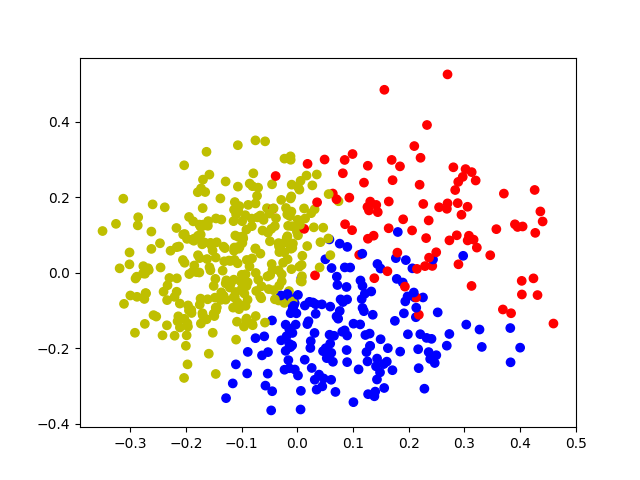
\includegraphics[scale=0.4]{kmeans_tokenizer2}
		\caption{El código utilizado para crear este diagrama fue escrito por \href{https://stackoverflow.com/questions/57626286/how-to-plot-text-clusters}{Matt L en StackOverflow}.}
	\end{subfigure}%
	\begin{subfigure}{.5\textwidth}
		\centering
		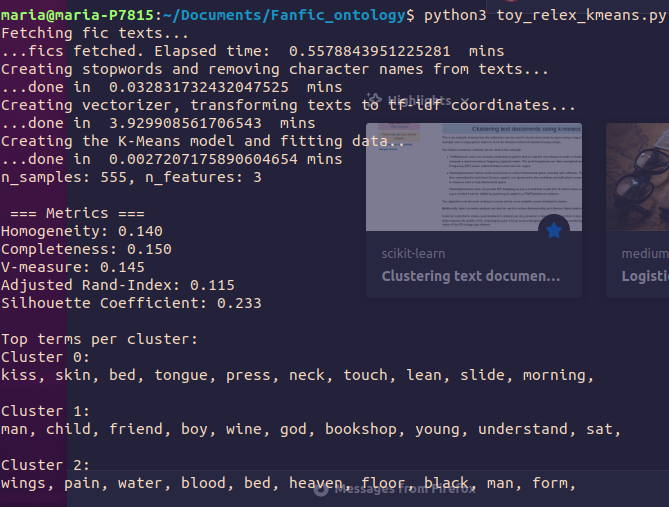
\includegraphics[scale=0.3]{ejecucion_kmeans_tokv2_0}
	\end{subfigure}
		
	\caption{A la derecha, ejecución de \textit{toy\_relex\_kmeans}, mostrando su evaluación. La homogeneidad se cumple cuando ningún cluster contiene miembros que pertenezcan a categorías distintas en los datos reales. La completitud se satisface si todos los miembros de una de las categorías reales pertenecen al mismo cluster. A la izquierda, el diagrama creado por el programa.}
	\label{fig:kmeanresult}
\end{figure}

Los resultados no son muy buenos. Aunque los términos de cada cluster parecen prometedores, ninguna métrica sube del 0.1, lo que indica que las categorías del clustering son sólo un poco mejores que haberlas asignado al azar, y que hay mucho solapamiento entre clusters.

Puesto que para crear el modelo he utilizado datos filtrados a propósito para modelar cada categoría tan bien como fuera posible, con la esperanza de poder usarlo como posible semilla para un sistema más general, esto supone un gran problema.

Busqué entonces otra estrategia, utilizando un modelo de temas más que uno de clustering. El modelado de temas con el algoritmo LDA parece también una buena opción para este problema, puesto que al contrario que el clustering clásico, LDA asigna a cada documento una distribución de temas en cada uno. Esto se ajusta a este análisis, puesto que aunque he intentado crear \textit{datasets} 'perfectos' que traten un único tipo de relación en cada uno, lo cierto es que lo normal en un relato es que estén mezcladas.

LDA es un algoritmo que descubre temas de forma no supervisada. Trabaja bajo la asunción de que cada documento es un conjunto de temas, y que cada tema es un conjunto de palabras. Empieza asignando cada a palabra a un conjunto al azar de temas, y en cada iteración mejora la asignación. 

Al igual que en el programa anterior, LDA requiere un preprocesado del texto, con lo que utilizo los dos \textit{tokenizers} del algoritmo de clustering. \textit{Scikit-Learn} carece de modelo LDA, por lo que utilizo el de la librería \textit{gensim}. LDA también trata los textos como un \textit{bag of words}, pero no es necesario vectorizarlos antes de usarlos para entrenar el modelo, que devolverá  lista de palabras por tema, junto con la probabilidad de que esa palabra pertenezca a dicho tema.

Tras preprocesar los textos de forma similar a como se hizo con clustering y entrenar el modelo LDA, se observan los resultados en la figura \ref{fig:topicresult1}.

\begin{figure}
	\begin{subfigure}{\textwidth}
		\hspace{-1cm}
		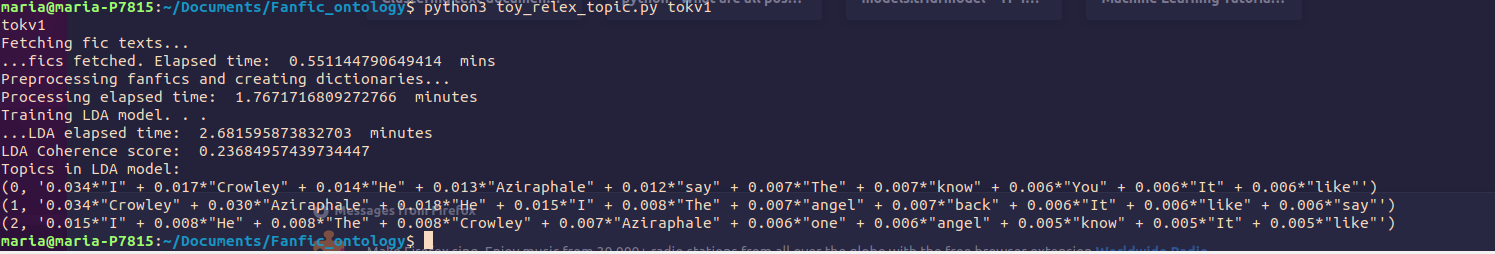
\includegraphics[scale=0.35]{ejecucion_topic_v1_0}
		\caption{Filtrado: sólo puntuación.}
		\label{fig:topicresult1}
	
	\end{subfigure}
	\begin{subfigure}{\textwidth}
		\hspace{-1cm}
		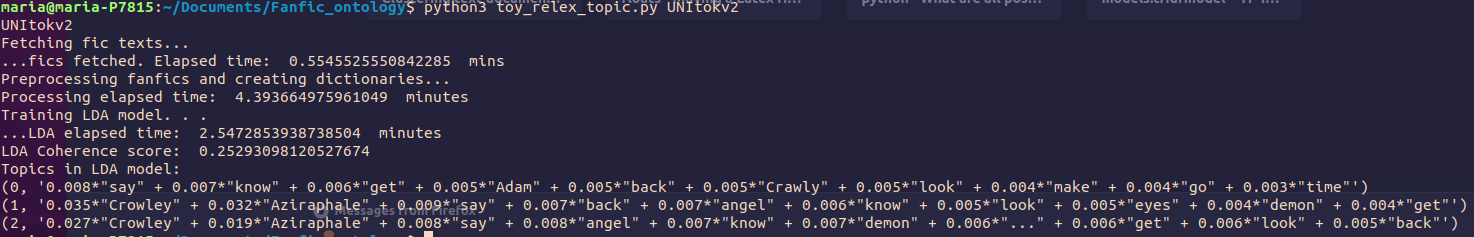
\includegraphics[scale=0.35]{ejecucion_topic_v2_0}
		\caption{Filtrado: puntuación, pronombres, determinantes, etc.}
		\label{fig:topicresult2}
	\end{subfigure}

	\caption{Ejecución de \textit{toy\_relex\_lda}, con distintos criterios de filtrado. Además se muestran los 10 términos más relevantes de cada tema, y su probabilidad de pertenecer a dicho tema.}

\end{figure}

Los resultados son un poco decepcionantes, pues ninguno de los 10 términos más relevantes por tema tiene siquiera un 0.1\% de probabilidad de pertenecer a su tema.
Tampoco es sorprende que no sean muy relevantes, pues aparecen muchos pronombres, determinantes e incluso algún número. Aprovechando el etiquetado de rol morfológico de NLTK, se retiran esas palabras y se crea un nuevo modelo, cuya ejecución está en la figura \ref{fig:topicresult2}.


Estos resultados, sin embargo, tampoco son muy convincentes. La puntuación de coherencia, que indica cómo de adecuado es el número de temas para los datos analizados, es 0.23 en el primer caso y 0.25 en el segundo. Es un resultado que se puede mejorar afinando los hiperparámetros de LDA, para lo cual se utiliza el programa \textit{topic\_evaluate.py}, que prueba diferentes valores para \textit{alpha} (densidad documento-tema) y \textit{beta} (densidad palabra-tema) del modelo LDA de \textit{gensim}. Los resultados de su ejecución se guardan en el archivo \textit{lda\_evaluation.csv}, y en la figura \ref{fig:lda_eval0} se puede ver que la puntuación de coherencia se puede mejorar bastante para tres temas con los hiperparámetros correctos, pero como evidencia la figura \ref{fig:lda_eval1}, queda muy lejos del 0.42 de coherencia que se puede conseguir si se permite subir el número de temas a nueve. No parece, por tanto, que este modelo sea el más adecuado para buscar las relaciones que se buscan.


\begin{figure}
	\centering
	\begin{subfigure}{\textwidth}
		%\hspace{-1cm}
		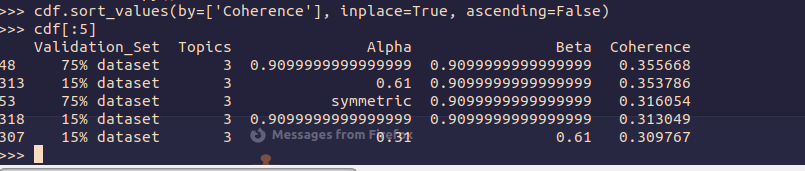
\includegraphics[scale=0.5]{lda_evaluate0}
		\caption{Mejores puntuaciones de coherencia para 3 temas.}
		\label{fig:lda_eval0}
		
	\end{subfigure}
	\begin{subfigure}{\textwidth}
		%\hspace{-1cm}
		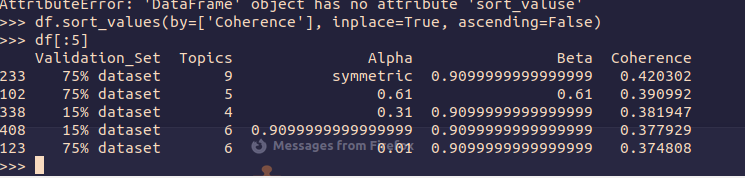
\includegraphics[scale=0.5]{lda_evaluate1}
		\caption{Parámetros con las mejores puntuaciones de coherencia de toda la prueba.}
		\label{fig:lda_eval1}
	\end{subfigure}
	
	\caption{Resultados de \textit{topic\_evaluate.py}, visualizados y ordenados con la ayuda de \textit{pandas}. Se pueden observar qué número de temas y qué hiperparámetros dan mejores puntuaciones de coherencia para el modelo LDA creado a partir del RFE dataset.}
	
\end{figure}



%\begin{itemize}
%	\item El modelo B tenía en cuenta sustantivos, adverbios y verbos.
%	\item El modelo C tenía en cuenta sustantivos, adjetivos y verbos.
%	\item El modelo D tenía en cuenta sustantivos, adverbios, adjetivos y verbos.
%\end{itemize}

%Además de utilizar distintas categorías morfológicas, también probé distintos tamaños para el set de entrenamiento, de modo que cada modelo tiene dos versiones: una entrenada con 5000 fanfics y otra entrenada con 10000.

%Para la evaluación de los modelos, simplemente los puse a clasificar textos nuevos, contando la cantidad de aciertos de cada uno y calculando el \textit{hit ratio} de cada uno. Los resultados aparecen en la primera tabla de la figura \ref{table:topic_evaluation}.

%\begin{gather*}
%hit\_ratio = %\frac{correct\_guesses}{total\_number\_of\_guesses}
%\end{gather*}

%\begin{figure}
%	\caption{Porcentaje de aciertos de cada modelo. Cada prueba se realizó tres veces.}
%	\label{table:topic_evaluation}
%	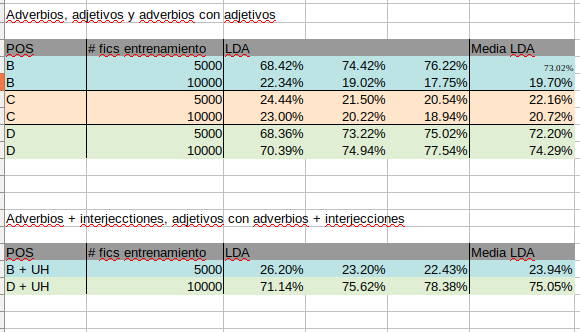
\includegraphics[scale=0.6]{topic_evaluate_table_v2}
%	\centering
%\end{figure}

%Las primeras pruebas mostraron que los modelos B y D eran los que arrojaban mejores resultados. Observando qué otras categorías morfológicas el \textit{tagger} de NLTK puede identificar, pensé que añadir interjecciones a los modelos podría aumentar su precisión. Llamé B+UH y D+UH a los modelos resultantes, y repetí las pruebas. Los resultados están en la segunda tabla de la figura \ref{table:topic_evaluation}.

%Curiosamente, el modelo D fue mejorado ligeramente teniendo en cuenta las interjecciones, pero el modelo B empeoró considerablemente.


\subsubsection{Correferencia con CoreNLP}
\label{sec:correferencia}
Tras varias pruebas con los algoritmos de clustering y LDA, encontré \textit{CorenNLP}, un servidor de Stanford NLP Group que realiza diversos tipos de extracción de información y análisis de lenguaje natural, entre ellos, resolución de correferencia.

Volviendo al ejemplo de Romeo y Julieta, una frase como \textit{'I love you', said Romeo}, extraída de un texto más largo en la que el contexto es que Romeo está hablando con Julieta, da poca información a un algoritmo que no es capaz de entender a qué personajes se refieren los pronombres \textit{I} y \textit{you}. Sin embargo, si se aplicase resolución de correferencia sobre el texto, a ojos del algoritmo la frase se convertiría en \textit{'Romeo love Juliette', said Romeo}, con lo que el algoritmo entiende mucho mejor qué está pasando en esta frase y a quiénes afecta.\label{nota:corref}

\textit{CoreNLP} da acceso a esa posibilidad. Aunque está programado en java, cuenta con un módulo de python llamado \textit{Stanza}, con lo que creé algunos programas para familiarizarme con su funcionamiento y la idea que quería desarrollar. El primero de estos programas, \textit{toy\_relex.py}, no hace más que buscar las frases que contengan el verbo 'to love' y al menos una entidad, elegida de antemano. El segundo programa, \textit{toy\_relex\_v2.py} expande este concepto usando \textit{CoreNLP}, utilizando tanto su función de identificación de entidades como la de solución de correferencia para obtener las 'cadenas de correferencia' del texto, utilizándolas para enlazar cada pronombre del texto con la entidad a la que se refiere. La idea sigue siendo seleccionar las frases que tengan el verbo \textit{'to love'}, pero en vez de quedarme únicamente con aquellas en las que se nombren explícitamente a un personaje, también me quedo con aquellas en las que los pronombres formen parte de una cadena de correferencia.

Para poder llevar a cabo todo esto, fue necesario estudiar con atención las propiedades de los objetos que utiliza \textit{Stanza}, que por suerte están bien \href{https://github.com/stanfordnlp/stanza/blob/master/doc/CoreNLP.proto}{documentadas}, y hacer muchas pruebas y visualización de datos, como se puede ver en las figuras \ref{fig:core_visualization_0} y \ref{fig:core_visualization_1}.


\begin{figure}
	\centering
	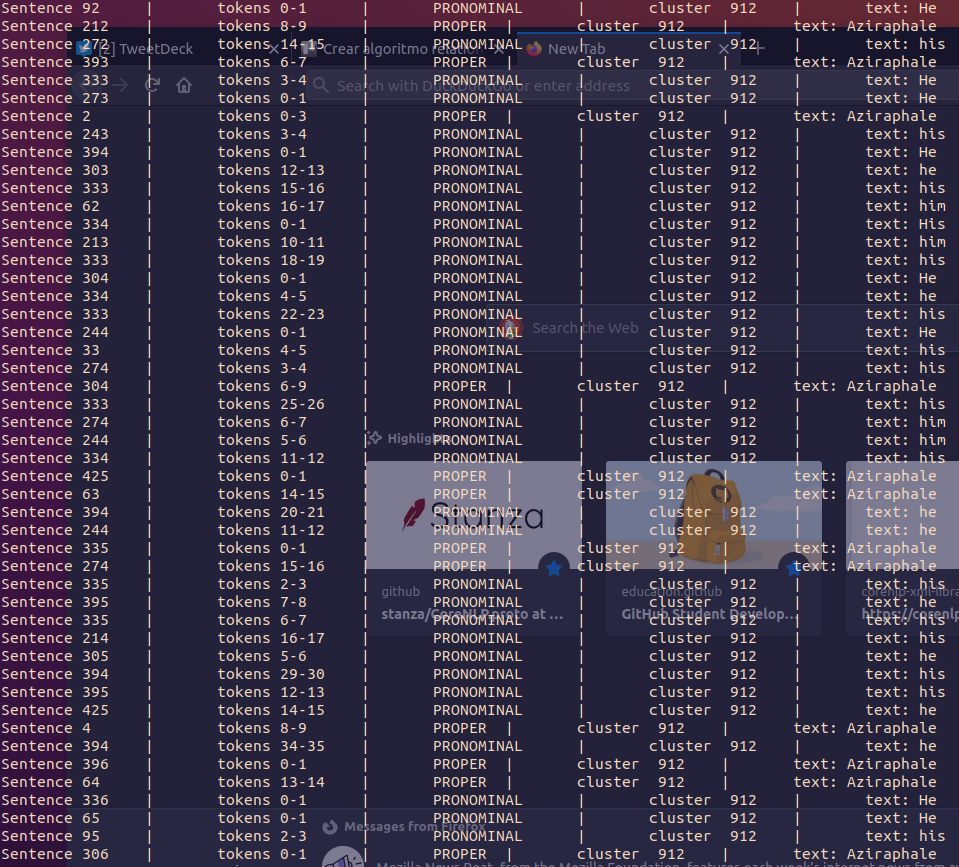
\includegraphics[scale=0.45]{core_vis_1}
	\caption{Visualización de la información proporcionada por \textit{CoreNLP}}
	\label{fig:core_visualization_0}
\end{figure}

\begin{figure}
	\centering
	\begin{subfigure}{.45\textwidth}
		\centering
		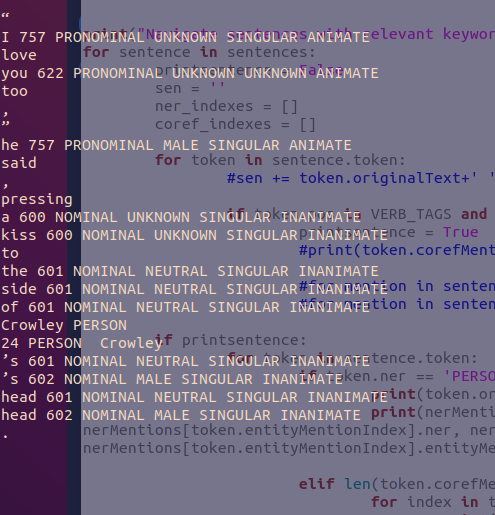
\includegraphics[scale=0.4]{core_vis_3}
	\end{subfigure}%
	\begin{subfigure}{.45\textwidth}
		\centering
		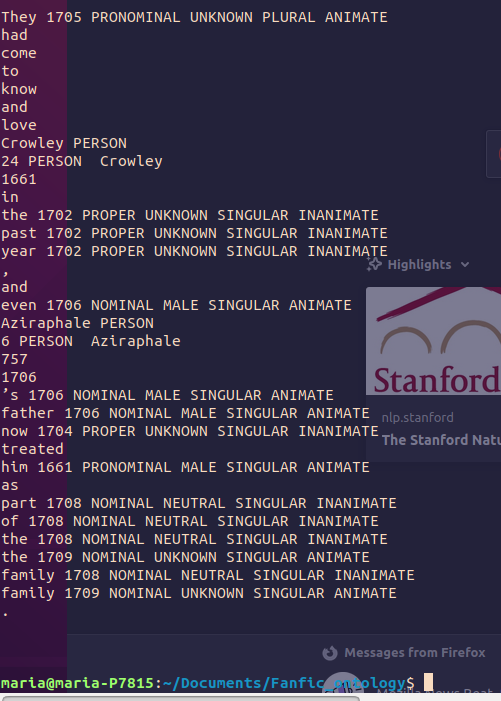
\includegraphics[scale=0.4]{core_vis_4}
	\end{subfigure}

	\caption{Visualización de frases particulares con anotaciones de correferencia de \textit{CoreNLP}}
	\label{fig:core_visualization_1}
\end{figure}

Mientras aprendía a manejar los objetos de \textit{Stanza} fui desarrollando distintos programas 

El objetivo es crear un programa que sea capaz de resumir la información proporcionada por CoreNLP de forma que sea útil para identificar relaciones entre personajes y probarlo con el RFE dataset.

El problema es que el RFE dataset es bastante grande, y CoreNLP tarda varias horas en analizarlo entero. Obviamente esto significa que es necesario guardar la información proporcionada por CoreNLP en un archivo. Puesto que dicha información viene encapsulada en un objeto \textit{Document} que no tiene una forma sencilla de ser almacenado como tal, creé un programa que, tras recoger las respuestas del servidor, resumía la información más relevante y la guardaba en dos archivos csv: fic\_characters.csv para los personajes junto con los identificadores dados por CoreNLP, y fic\_sentences para almacenar cada fanfic frase a frase, cada una con el ID de su fanfic, su sentimiento, y los identificadores de los personajes mencionadas en ellas.


Otras movidas que he hecho han sido observar la frecuencia de ciertos elementos lingüísticos en las frases en las que se mencionan específicamente a dos personajes, intentando buscar algún patrón entre ellos. Así que cogí el RFE dataset, utilicé CoreNLP combinado con NERTagger para obtener los personajes y las menciones pronominales a los mismos, y guardé los datos en 
Estos dos archivos me servirán como base de datos con la que hacer pruebas e intentar buscar algún patrón que me permita identificar relaciones entre personajes. Traté de buscar patrones en los verbos, adjetivos, bigramas y trigramas más frecuentes en las frases que mencionan dos personajes, y más en general, en el conjunto de relatos clasificados como romance, amistad o enemistad.

\todo{explicar búsqueda de patrones en datos Corenlp}
Ejemplos de la distribución de frecuencia de lo verbos en el RFE dataset:

\begin{figure}
	\centering
	\begin{subfigure}{\textwidth}
		%\hspace{-1cm}
		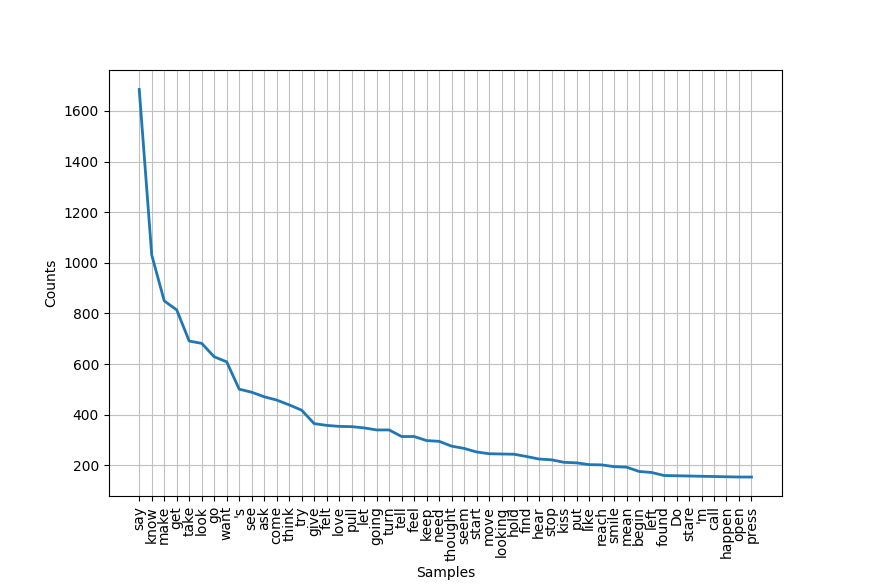
\includegraphics[scale=0.7]{r_verbs_0}
		\caption{Verbos más frecuentes en el dataset de romance.}
		\label{fig:r_verb_freq_in_dataset}
		
	\end{subfigure}
	\begin{subfigure}{\textwidth}
		%\hspace{-1cm}
		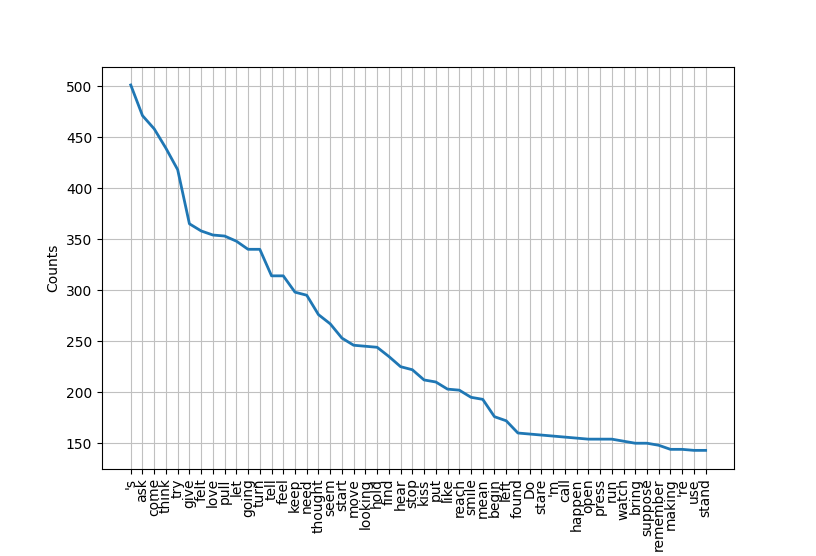
\includegraphics[scale=0.7]{r_verbs_1}
		\caption{Verbos más frecuentes en el dataset de romance, tras retirar los más comunes.}
		\label{fig:r_verb_freq_removed}
	\end{subfigure}
	
	%\caption{...}
	
\end{figure}


\begin{figure}
	\centering
	\begin{subfigure}{\textwidth}
		%\hspace{-1cm}
		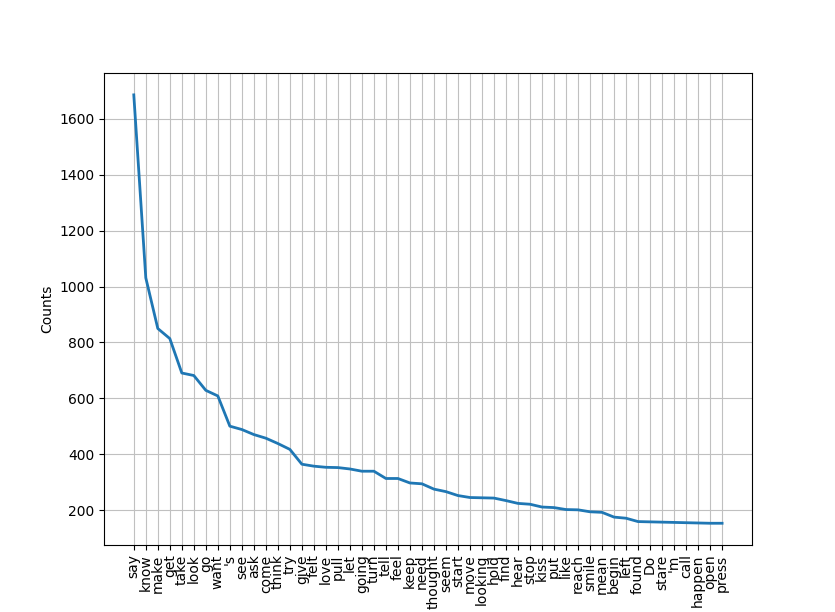
\includegraphics[scale=0.7]{f_verbs_0}
		\caption{Verbos más frecuentes en el dataset de amistad.}
		\label{fig:f_verb_freq_in_dataset}
		
	\end{subfigure}
	\begin{subfigure}{\textwidth}
		%\hspace{-1cm}
		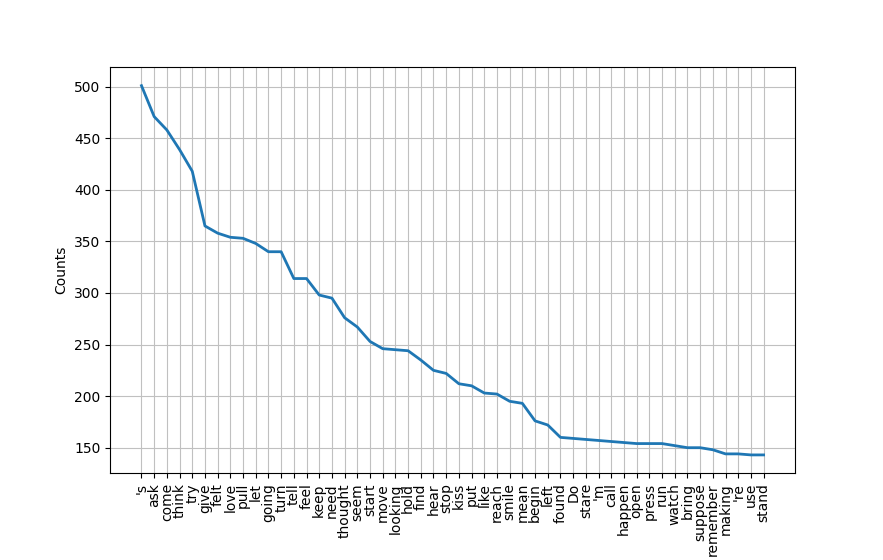
\includegraphics[scale=0.7]{f_verbs_1}
		\caption{Verbos más frecuentes en el dataset de amistad, tras retirar los más comunes.}
		\label{fig:f_verb_freq_removed}
	\end{subfigure}
	
	%\caption{...}
	
\end{figure}


\begin{figure}
	\centering
	\begin{subfigure}{\textwidth}
		%\hspace{-1cm}
		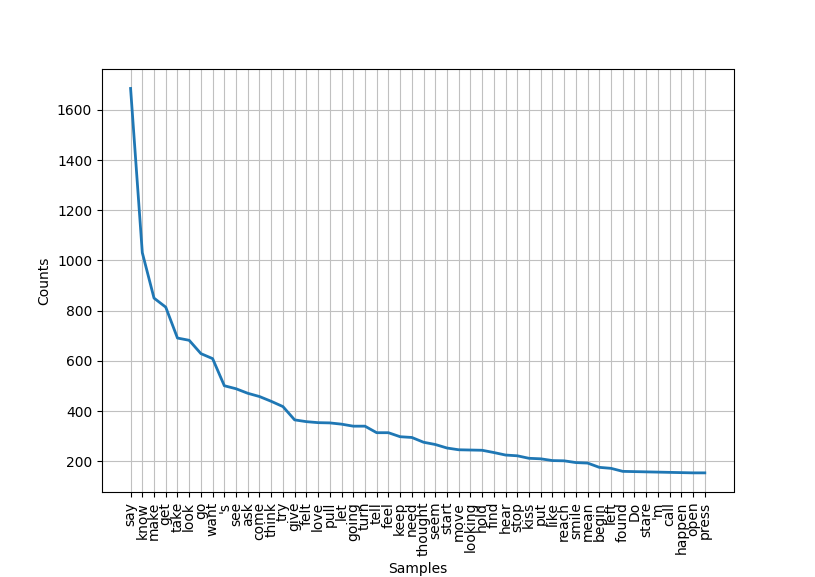
\includegraphics[scale=0.7]{e_verbs_0}
		\caption{Verbos más frecuentes en el dataset de enemistad.}
		\label{fig:e_verb_freq_in_dataset}
		
	\end{subfigure}
	\begin{subfigure}{\textwidth}
		%\hspace{-1cm}
		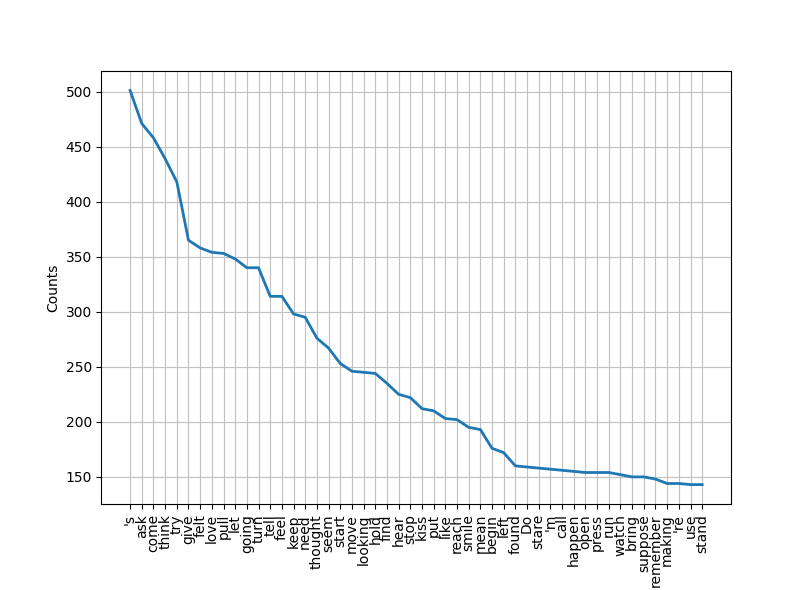
\includegraphics[scale=0.7]{e_verbs_1}
		\caption{Verbos más frecuentes en el dataset de enemistad, tras retirar los más comunes.}
		\label{fig:e_verb_freq_removed}
	\end{subfigure}
	
	%\caption{...}
	
\end{figure}

En los tres casos los verbos más repetidos fueron verbos muy comunes en inglés, como "say", "go", "get", "make", "look", etc. de modo que para eliminar ruido hice otro análisis eliminándolos:

También comparé bigramas y trigramas, probando con el likelihood y pmi como criterios:

\begin{figure}
	\centering
	\begin{subfigure}{\textwidth}
		%\hspace{-1cm}
		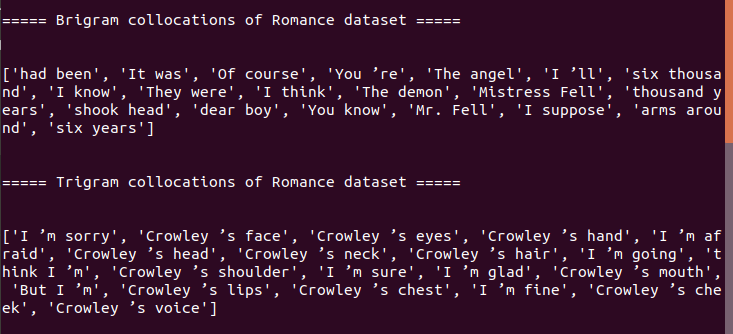
\includegraphics[scale=0.5]{r_btrigrams_lik}
		\caption{Bigramas y trigramas con mayor likelihood en el dataset de romance}
		\label{fig:r_btrigram_lik}
		
	\end{subfigure}
	\begin{subfigure}{\textwidth}
		%\hspace{-1cm}
		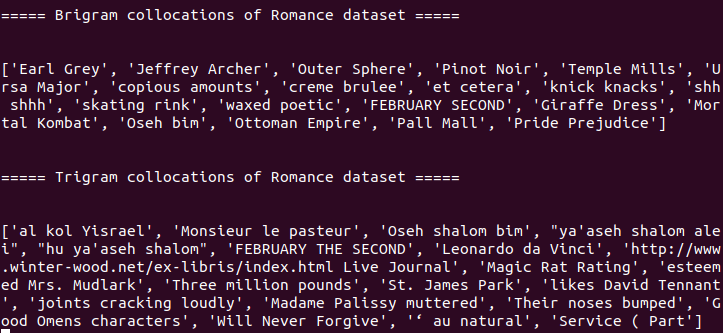
\includegraphics[scale=0.5]{r_btrigrams_pmi}
		\caption{Bigramas y trigramas con mayor pmi en el dataset de romance}
		\label{fig:r_btrigram_pmi}
	\end{subfigure}
	
	%\caption{...}
	
\end{figure}

\begin{figure}
	\centering
	\begin{subfigure}{\textwidth}
		%\hspace{-1cm}
		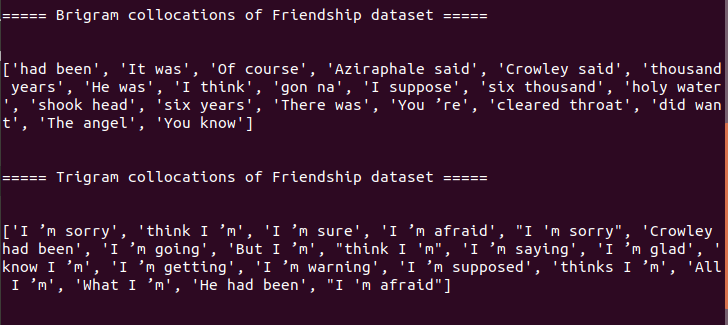
\includegraphics[scale=0.5]{f_btrigrams_lik}
		\caption{Bigramas y trigramas con mayor likelihood en el dataset de amistad}
		\label{fig:f_btrigram_lik}
		
	\end{subfigure}
	\begin{subfigure}{\textwidth}
		%\hspace{-1cm}
		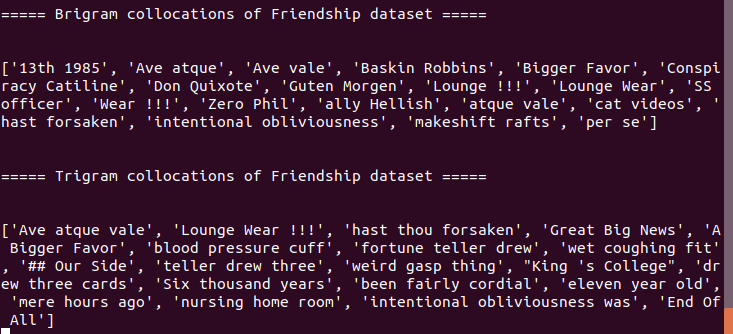
\includegraphics[scale=0.5]{f_btrigrams_pmi}
		\caption{Bigramas y trigramas con mayor pmi en el dataset de amistad}
		\label{fig:f_btrigram_pmi}
	\end{subfigure}
	
	%\caption{...}
	
\end{figure}

\begin{figure}
	\centering
	\begin{subfigure}{\textwidth}
		%\hspace{-1cm}
		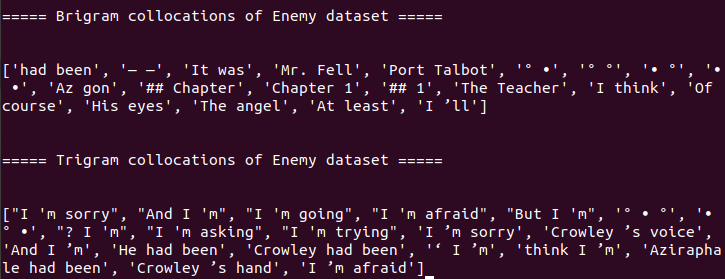
\includegraphics[scale=0.5]{e_btrigrams_lik}
		\caption{Bigramas y trigramas con mayor likelihood en el dataset de enemistad}
		\label{fig:e_btrigram_lik}
		
	\end{subfigure}
	\begin{subfigure}{\textwidth}
		%\hspace{-1cm}
		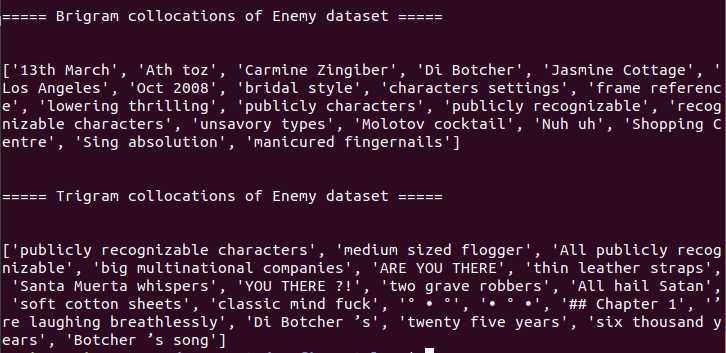
\includegraphics[scale=0.5]{e_btrigrams_pmi}
		\caption{Bigramas y trigramas con mayor pmi en el dataset de enemistad}
		\label{fig:e_btrigram_pmi}
	\end{subfigure}
	
	%\caption{Resultados de \textit{topic\_evaluate.py}, visualizados y ordenados con la ayuda de \textit{pandas}. Se pueden observar qué número de temas y qué hiperparámetros dan mejores puntuaciones de coherencia para el modelo LDA creado a partir del RFE dataset.}
	
\end{figure}


%\begin{figure}
%	\centering
%	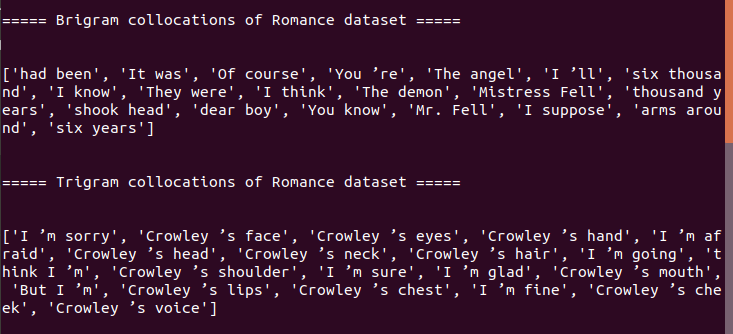
\includegraphics[scale=0.7]{r_btrigrams_lik}
%	\caption{Bigramas y trigramas con mayor likelihood en el dataset de romance.}
%	\label{fig:r_btrigram_lik}
%\end{figure}

%\begin{figure}
%	\centering
%	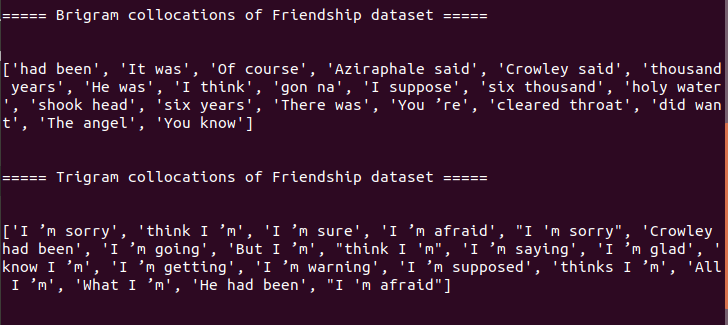
\includegraphics[scale=0.7]{f_btrigrams_lik}
%	\caption{Bigramas y trigramas con mayor likelihood en el dataset de amistad.}
%	\label{fig:f_btrigram_lik}
%\end{figure}

%\begin{figure}
%	\centering
%	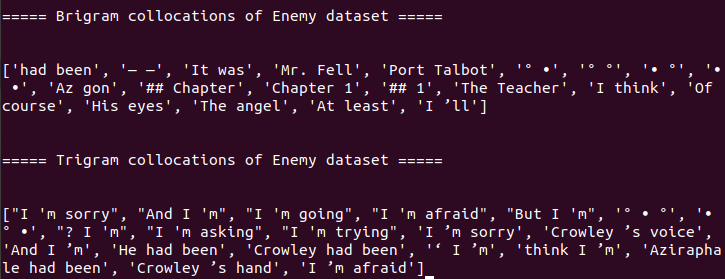
\includegraphics[scale=0.65]{e_btrigrams_lik}
%	\caption{Bigramas y trigramas con mayor likelihood en el dataset de enemistad.}
%	\label{fig:e_btrigram_lik}
%\end{figure}

Tras haber realizado este análisis con los relatos de romance, amistad y enemistad en general, decidí probar lo mismo pero utilizando únicamente las frases en las que se mencione a dos personajes en concreto, en vez de todas las frases del relato:

\begin{figure}
	\centering
	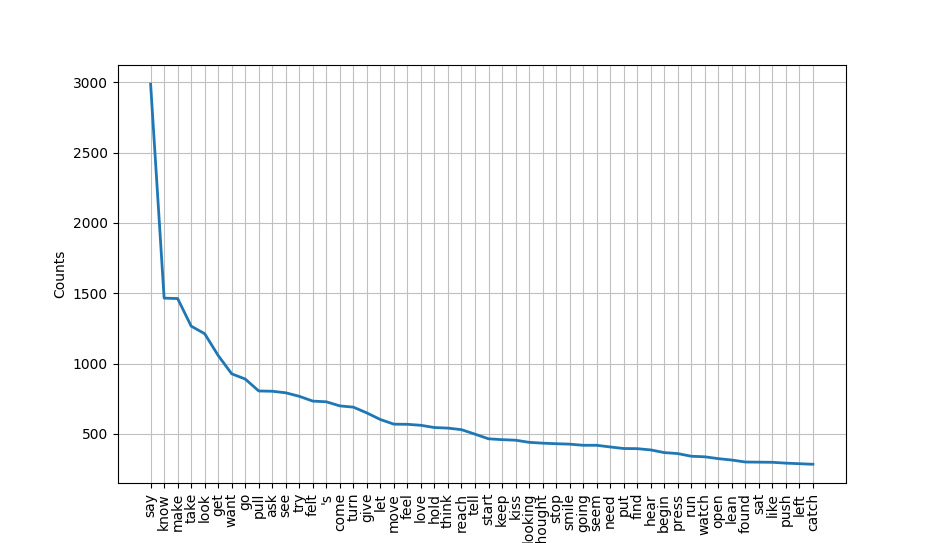
\includegraphics[scale=0.6]{ac_rverbs_2}
	\caption{Verbos más frecuentes en el dataset de romance en las frases que mencionan a dos personajes concretos.}
	\label{fig:r_verb_freq_in_character_mentions}
\end{figure}


\begin{figure}
	\centering
	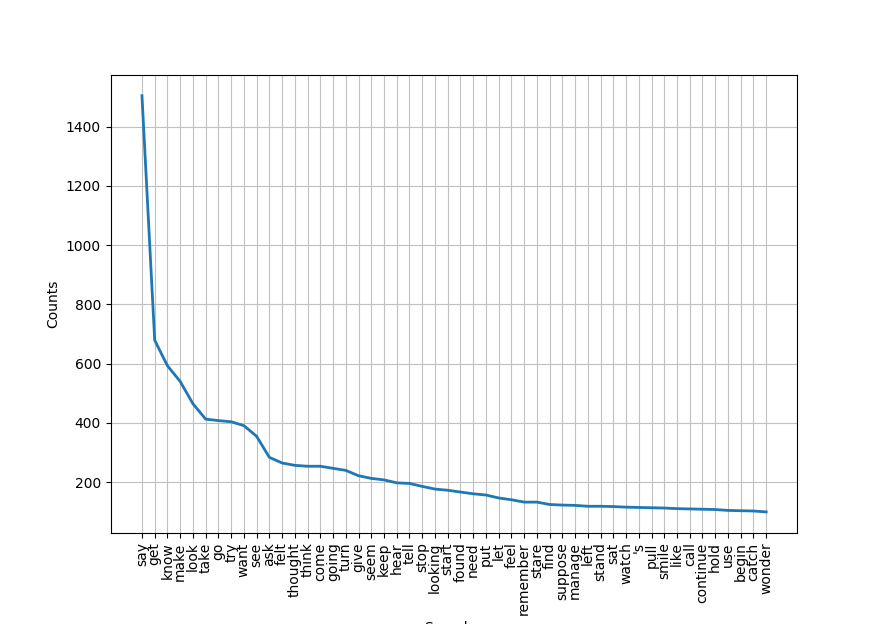
\includegraphics[scale=0.6]{ac_fverbs_2}
	\caption{Verbos más frecuentes en el dataset de amsitad en las frases que mencionan a dos personajes concretos.}
	\label{fig:f_verb_freq_in_character_mentions}
\end{figure}


\begin{figure}
	\centering
	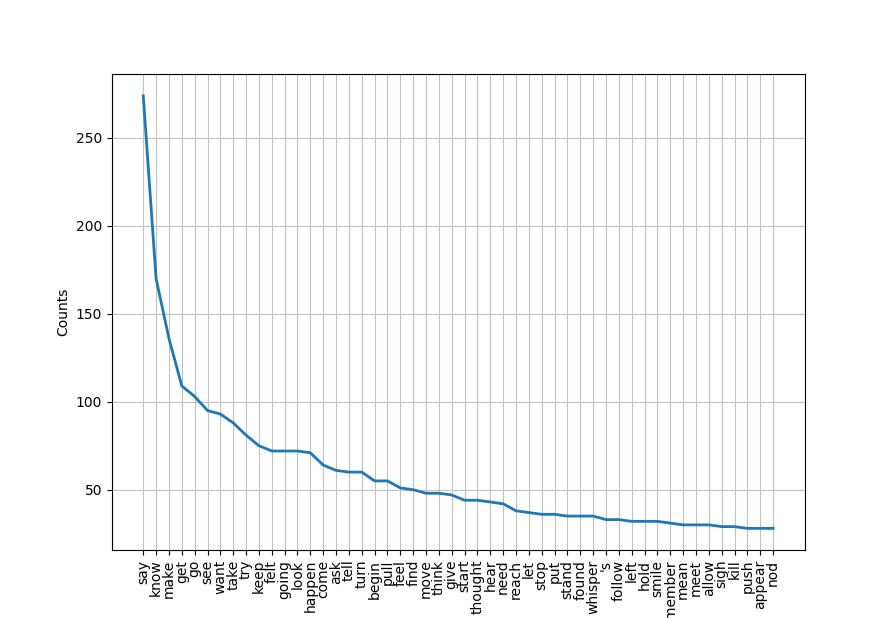
\includegraphics[scale=0.6]{crowhas_everbs_0}
	\caption{Verbos más frecuentes en el dataset de enemistad en las frases que mencionan a dos personajes concretos.}
	\label{fig:e_verb_freq_in_character_mentions}
\end{figure}






\section{EVALUACIÓN DEL SISTEMA}


\section{REFERENCIAS}




\bibliographystyle{alpha}
\singlespacing
%\bibliography{ejemplo}
\bibliography{bib_tfg}


\end{document}


% Local Variables:
% coding: utf-8
% mode: flyspell
% ispell-local-dictionary: "castellano8"
% mode: latex
% End:
